%%%%%%%%%%%%%%%%%%%%%%%%%%%%%%%%%%%%%%%%%%%%%%%%%%%%%%%%%%%%%%%%%%%%%%
% Overleaf (WriteLaTeX) Example: Molecular Chemistry Presentation
%
% Source: http://www.overleaf.com
%
% In these slides we show how Overleaf can be used with standard 
% chemistry packages to easily create professional presentations.
% 
% Feel free to distribute this example, but please keep the referral
% to overleaf.com
% 
%%%%%%%%%%%%%%%%%%%%%%%%%%%%%%%%%%%%%%%%%%%%%%%%%%%%%%%%%%%%%%%%%%%%%%

\documentclass{beamer}

\mode<presentation>
{
  \usetheme{Madrid}       % or try default, Darmstadt, Warsaw, ...
  \usecolortheme{default} % or try albatross, beaver, crane, ...
  \usefonttheme{default}    % or try default, structurebold, ...
  \setbeamertemplate{navigation symbols}{}
  \setbeamertemplate{caption}[numbered]
} 

\usepackage[english]{babel}
\usepackage[utf8x]{inputenc}
\usepackage{graphicx}
\usepackage{hyperref}
  \hypersetup{colorlinks=true}
  \hypersetup{urlcolor=blue}
  \hypersetup{linkcolor = .}
\usepackage{xcolor}
\usepackage{siunitx}
  \sisetup{separate-uncertainty = true}
\usepackage{physics}
\usepackage[font=small,labelfont=bf]{caption}
\usepackage{subcaption}
\usepackage[en-GB]{datetime2}
\usepackage{overpic}
\usepackage{feynmp}
\DeclareGraphicsRule{*}{mps}{*}{}
\usepackage{scalerel}
\newcommand{\mylbrace}[2]{\vspace{#2pt}\hspace{6pt}\scaleleftright[\dimexpr5pt+#1\dimexpr0.06pt]{\lbrace}{\rule[\dimexpr2pt-#1\dimexpr0.5pt]{-4pt}{#1pt}}{.}}
\newcommand{\myrbrace}[2]{\vspace{#2pt}\scaleleftright[\dimexpr5pt+#1\dimexpr0.06pt]{.}{\rule[\dimexpr2pt-#1\dimexpr0.5pt]{-4pt}{#1pt}}{\rbrace}\hspace{6pt}}

% Here's where the presentation starts, with the info for the title slide
\title[$B^\pm\to(K^+K^-\pi^+\pi^-)_Dh^\pm$]{Determination of the CKM angle \texorpdfstring{$\gamma$}{gamma} in \texorpdfstring{$B^\pm\to(K^+K^-\pi^+\pi^-)_Dh^\pm$}{B to K+K-pi+pi-} decays}

\author{\textbf{Martin Tat} \hspace{0.54em} Guy Wilkinson \hspace{0.54em} Sneha Malde}
\institute{\normalsize University of Oxford \\ \vspace{0.3cm} \normalsize B2OC Meeting \vspace{-0.2cm}}
\date{4th November 2021}

\titlegraphic{
\includegraphics[height = 2cm]{lhcb.jpg}\hspace{2cm}~%
              
\includegraphics[height = 2cm]{OxfordLogo.pdf}}

\begin{document}

\begin{frame}
  \titlepage
\end{frame}

% These three lines create an automatically generated table of contents.
\begin{frame}{Outline}
  \tableofcontents
\end{frame}

\section{Introduction to the CKM angle \texorpdfstring{$\gamma$}{gamma}}
\begin{frame}{$\gamma$ and the unitary triangle}
  \begin{itemize}
    \setlength\itemsep{1.0em}
    \item{Unitarity of CKM matrix: $V_{ud}V^*_{ub} + V_{cd}V^*_{cb} + V_{td}V^*_{tb} = 0\implies$}
    \end{itemize}
    \begin{center}
    $\gamma = \text{arg}\Big(-\frac{V_{ud}V^*_{ub}}{V_{cd}V^*_{cb}}\Big)$
  \end{center}
  \begin{itemize}
    \item{Only CKM angle accessible at tree level $\implies$}
    \begin{itemize}
      \item{Negligible theoretical uncertainties}
      \item{Ideal Standard Model benchmark}
      \item{Compare with indirect measurements}
    \end{itemize}
  \end{itemize}
  \vspace{-0.2cm}
  \begin{figure}
    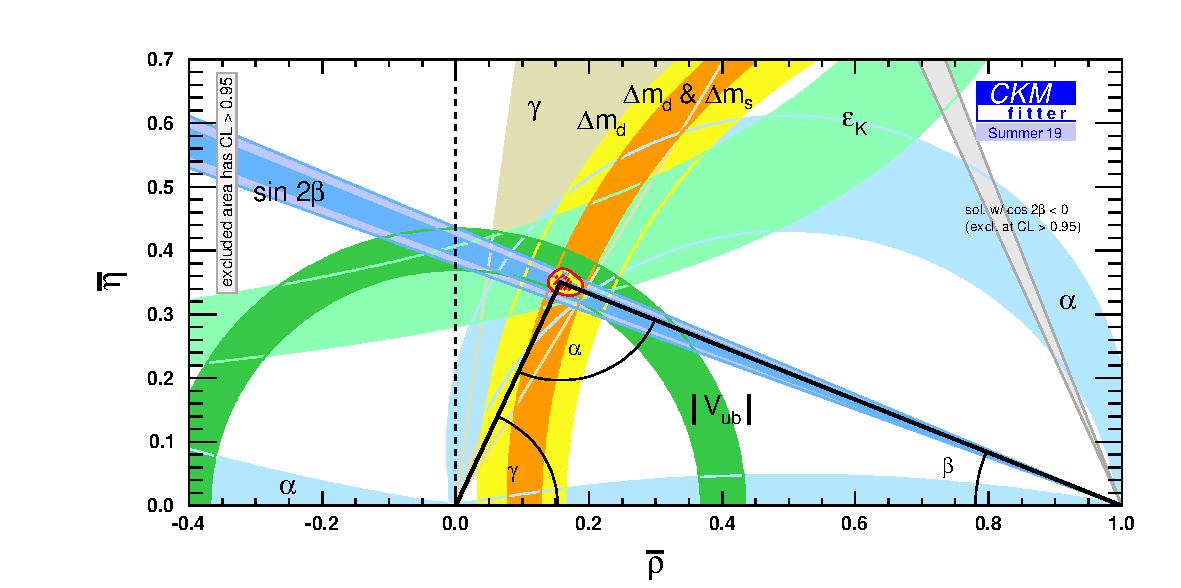
\includegraphics[width = 0.70\textwidth]{Plots/ckmfitter2.pdf}
  \end{figure}
  \vspace{-0.5cm}
  \begin{center}
    \tiny{CKMfitter Group (J. Charles et al.), Eur. Phys. J. C41, 1-131 (2005)}
  \end{center}
\end{frame}

\begin{frame}{Sensitivity through interference}
  \begin{figure}[H]
    \centering
    \vspace{0.3cm}
    \begin{subfigure}{0.5\textwidth}
      \centering
      \begin{fmffile}{fgraph/fgraph_BtoDK1}
        \setlength{\unitlength}{0.4cm}
        \begin{fmfgraph*}(6,6)
          \fmfstraight
          \fmfleft{i1,B,i2,t1,t2,t3,t9,t10}
          \fmfright{o1,D,o2,t4,t5,o3,K,o4}
          \fmflabel{$\bar{u}$}{i1}
          \fmflabel{$b$}{i2}
          \fmfv{l.d=20,l.a=180,l={$B^-$\mylbrace{30}{-8}}}{B}
          \fmflabel{$\bar{u}$}{o1}
          \fmflabel{$c$}{o2}
          \fmflabel{$\bar{u}$}{o3}
          \fmflabel{$s$}{o4}
          \fmfv{l.d=15,l.a=0,l={\myrbrace{30}{-12}}$D^0$}{D}
          \fmfv{l.d=15,l.a=0,l={\myrbrace{30}{11}}$K^-$}{K}
          \fmf{fermion}{o1,i1}
          \fmf{fermion,tension=1.5}{i2,v1}
          \fmf{fermion}{v1,o2}
          \fmf{phantom,tension=1.5}{t9,v2}
          \fmf{boson,label=$W$,label.side=left,tension=0}{v1,v2}
          \fmf{fermion}{v2,o4}
          \fmf{fermion}{o3,v2}
        \end{fmfgraph*}
      \end{fmffile}
      \vspace{0.5cm}
      \caption{$B^-\to D^0K^-$}
    \end{subfigure}%
    \begin{subfigure}{0.5\textwidth}
      \centering
      \begin{fmffile}{fgraph/fgraph_BtoDK2}
        \setlength{\unitlength}{0.4cm}
        \begin{fmfgraph*}(6,6)
          \fmfstraight
          \fmfleft{i1,t1,t2,B,t9,t10,i2}
          \fmfright{o1,K,o2,t4,t5,o3,D,o4}
          \fmflabel{$\bar{u}$}{i1}
          \fmflabel{$b$}{i2}
          \fmfv{l.d=20,l.a=180,l={$B^-$\mylbrace{100}{-8}}}{B}
          \fmflabel{$\bar{u}$}{o1}
          \fmflabel{$s$}{o2}
          \fmflabel{$\bar{c}$}{o3}
          \fmflabel{$u$}{o4}
          \fmfv{l.d=15,l.a=0,l={\myrbrace{30}{13}}$\bar{D^0}$}{D}
          \fmfv{l.d=15,l.a=0,l={\myrbrace{30}{-13}}$K^-$}{K}
          \fmf{fermion}{o1,i1}
          \fmf{fermion,tension=1.5}{i2,v1}
          \fmf{fermion}{v1,o4}
          \fmf{phantom,tension=1.5}{t2,v2}
          \fmf{boson,label=$W$,label.side=left,tension=0}{v1,v2}
          \fmf{fermion}{v2,o2}
          \fmf{fermion}{o3,v2}
        \end{fmfgraph*}
      \end{fmffile}
      \vspace{0.5cm}
      \caption{$B^-\to\bar{D^0}K^-$}
    \end{subfigure}
  \end{figure}
  \begin{itemize}
    \item{Superposition of $D^0$ and $\bar{D^0}$}
    \item{$b\to u\bar{c}s$ and $b\to c\bar{u}s$ interference $\to$ Sensitivity to $\gamma$}
  \end{itemize}
  \begin{center}
    $\mathcal{A}(B^-) = \mathcal{A}(D^0) + r_Be^{i(\delta_B - \gamma)}\mathcal{A}(\bar{D^0})$ \\
    $\mathcal{A}(B^+) = \mathcal{A}(\bar{D^0}) + r_Be^{i(\delta_B + \gamma)}\mathcal{A}(D^0)$ \\
  \end{center}
\end{frame}

\begin{frame}{Measurement of $\gamma$ from $B^\pm\to DK^\pm$, $D\to K^+K^-\pi^+\pi^-$}
  \vspace{0.0cm}
  \vspace{0.5cm}
  \begin{itemize}
    \setlength\itemsep{1.2em}
    \item{First proposed by J. Rademacker and G. Wilkinson}
    \begin{itemize}
      \item{\href{https://arxiv.org/abs/hep-ph/0611272}{arXiv:hep-ph/0611272}}
      \item{Amplitude model by FOCUS}
      \item{Expected $\gamma$ precision with $1000$ candidates: $14^\circ$}
    \end{itemize}
    \item{CLEO amplitude analysis}
    \begin{itemize}
      \item{\href{https://arxiv.org/abs/1201.5716}{arXiv:1201.5716}}
      \item{Expected $\gamma$ precision with $2000$ candidates: $11^\circ$}
    \end{itemize}
    \item{State of the art amplitude analysis by LHCb :}
    \begin{itemize}
      \item{\href{https://cds.cern.ch/record/2648586?ln=en}{LHCb-PAPER-2018-041}}
      \item{Use to develop efficient binning scheme}
    \end{itemize}
  \end{itemize}
\end{frame}

\section{Binned \texorpdfstring{$\gamma$}{gamma} analysis of the \texorpdfstring{$D\to K^+K^-\pi^+\pi^-$}{D->KKpipi} mode}
\begin{frame}{The $D\to K^+K^-\pi^+\pi^-$ decay}
  \begin{center}
    {\huge Binned $\gamma$ analysis of the $D\to K^+K^-\pi^+\pi^-$ mode}
  \end{center}
\end{frame}

\begin{frame}{Binned measurement of $\gamma$}
  \begin{itemize}
    \setlength\itemsep{0.5em}
    \item{Final measurement will be \underline{model-independent}}
    \begin{itemize}
      \item{Poor binning reduces statistical sensitivity $\to$ No bias!}
    \end{itemize}
    \item{Need strong phases of $D$ decay $\to$ Measure at BESIII}
    \item{LHCb-PAPER-2020-019: $B^\pm\to Dh^\pm$, $D\to K_S^0 h^+h^-$}
    \begin{itemize}
      \item{Single most precise measurement: $\gamma = (68.7^{+5.2}_{-5.1})^\circ$}
    \end{itemize}
  \end{itemize}
  \begin{figure}
    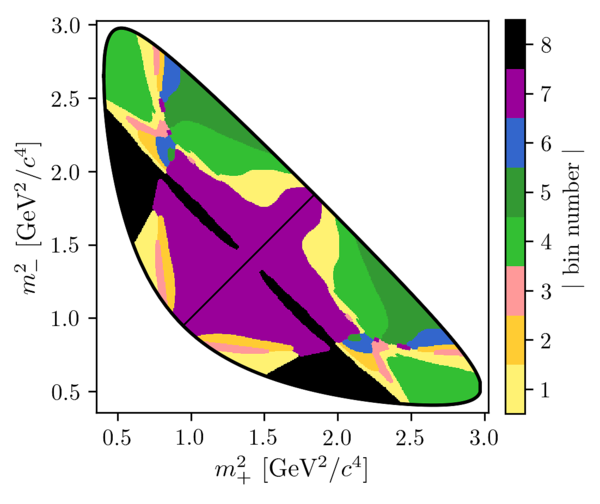
\includegraphics[height = 4cm]{Plots/KsPiPi_optimal.png}
    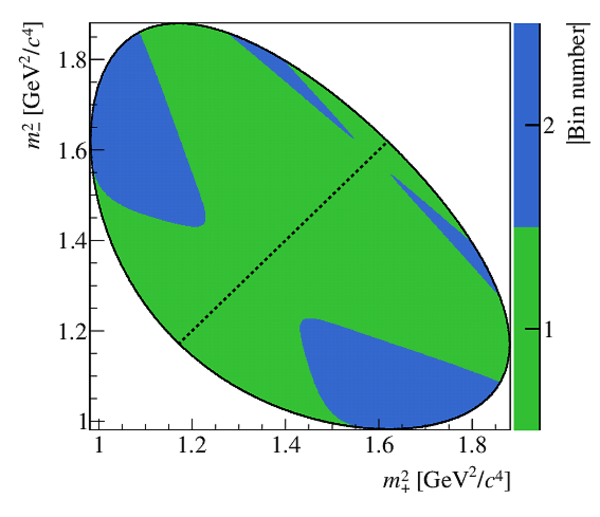
\includegraphics[height = 4cm]{Plots/KsKK_binning.png}
  \end{figure}
\end{frame}

\begin{frame}{The BPGGSZ method}
  \begin{itemize}
    \item{$B^\pm\to Dh^\pm$ amplitude:}
  \end{itemize}
  \begin{center}
    $\mathcal{A}(B^-) = \mathcal{A}(D^0) + r_Be^{i(\delta_B - \gamma)}\mathcal{A}(\bar{D^0})$ \\
    $\mathcal{A}(B^+) = \mathcal{A}(\bar{D^0}) + r_Be^{i(\delta_B + \gamma)}\mathcal{A}(D^0)$ \\
  \end{center}
  \begin{itemize}
    \item{$\mathcal{A}(D^0)$ and $\mathcal{A}(\bar{D^0})$ depend on $D$ phase space}
    \item{Strong-phase difference of $D^0$ and $\bar{D^0}$ decays inaccessible at LHCb}
    \item{Model-independent measurement: Integrate over bins of phase space}
  \end{itemize}
  \begin{block}{Event yield in bin $i$}
    $N^-_i = h_{B^-}\Big(F_i + \big(x_-^2 + y_-^2\big)\bar{F_i} + 2\sqrt{F_i\bar{F_i}}\big(x_-c_i + y_-s_i\big)\Big)$
    $N^+_{-i} = h_{B^+}\Big(F_i + \big(x_+^2 + y_+^2\big)\bar{F_i} + 2\sqrt{F_i\bar{F_i}}\big(x_+c_i + y_+s_i\big)\Big)$
  \end{block}
\end{frame}

\begin{frame}{The BPGGSZ method}
  \begin{block}{Event yield in bin $i$}
    \scriptsize
    $N^-_i = h_{B^-}\big(F_i + (x_-^2 + y_-^2)\bar{F_i} + 2\sqrt{F_i\bar{F_i}}(x_-c_i + y_-s_i)\big)$ \\
    $N^+_{-i} = h_{B^+}\big(F_i + (x_+^2 + y_+^2)\bar{F_i} + 2\sqrt{F_i\bar{F_i}}(x_+c_i + y_+s_i)\big)$
  \end{block}
  \begin{itemize}
    \item{CP observables:}
    \begin{itemize}
      \item{$x_\pm^{DK} = r_B^{DK}\cos(\delta_B^{DK}\pm\gamma)$, \quad $y_\pm^{DK} = r_B^{DK}\sin(\delta_B^{DK}\pm\gamma)$}
      \item{$x_\xi^{D\pi} = \Re(\xi^{D\pi})$, $y_\xi^{D\pi} = \Im(\xi^{D\pi})$ $\quad\quad\Big(\xi^{D\pi} = \frac{r_B^{D\pi}}{r_B^{DK}}e^{i(\delta_B^{D\pi} - \delta_B^{DK})}\Big)$}
    \end{itemize}
    \item{Fractional bin yield:}
    \begin{itemize}
      \item{$F_i = \frac{\int_i\dd{\Phi}|\mathcal{A}(D^0)|^2}{\sum_j\int_j\dd{\Phi}\abs{\mathcal{A}(D^0)}^2}$}
      \item{Floated in the fit, mostly constrained by $B^\pm\to D\pi^\pm$}
    \end{itemize}
  \end{itemize}
  \begin{itemize}
    \item{Amplitude averaged strong phases from BESIII:}
    \begin{center}
      $c_i = \frac{\int_i\dd{\Phi}|\mathcal{A}(D^0)||\mathcal{A}(\bar{D^0})|\cos(\delta_D)}{\sqrt{\int_i\dd{\Phi}\abs{\mathcal{A}(D^0)}^2\int_i\dd{\Phi}\abs{\mathcal{A}(\bar{D^0})}^2}}$ \quad $s_i = \frac{\int_i\dd{\Phi}|\mathcal{A}(D^0)||\mathcal{A}(\bar{D^0})|\sin(\delta_D)}{\sqrt{\int_i\dd{\Phi}\abs{\mathcal{A}(D^0)}^2\int_i\dd{\Phi}\abs{\mathcal{A}(\bar{D^0})}^2}}$
    \end{center}
  \end{itemize}
\end{frame}

\section{Binning scheme}
\begin{frame}{Binning Scheme}
  \begin{center}
    {\huge Binning scheme}
  \end{center}
\end{frame}

\begin{frame}{Binning scheme requirements}
  \vspace{0.0cm}
  {\Large A binning scheme must satisfy the following:}
  \begin{itemize}
    \item{Minimal dilution of strong phases when integrating over bins}
    \item{Enhance interference between $B^\pm\to D^0h^\pm$ and $B^\pm\to\bar{D^0}h^\pm$}
  \end{itemize}
  \vspace{0.4cm}
  {\Large How to bin a 5-dimensional phase space?}
  \begin{itemize}
    \item{Generate C++ code for LHCb amplitude model using AmpGen\footnote{\href{https://github.com/GooFit/AmpGen}{AmpGen} by Tim Evans}}
    \item{For each $B^\pm$ candidate, calculate}
  \end{itemize}
  \begin{center}
    {\Large $\frac{\mathcal{A}(D^0)}{\mathcal{A}(\bar{D^0})} = r_De^{i\delta_D}$}
  \end{center}
  \begin{itemize}
    \item{Bin along $\delta_D$ and $r_D$, maximize $Q$-value to optimize}
  \end{itemize}
\end{frame}

\begin{frame}{Binning scheme}
  \begin{figure}
    \centering
    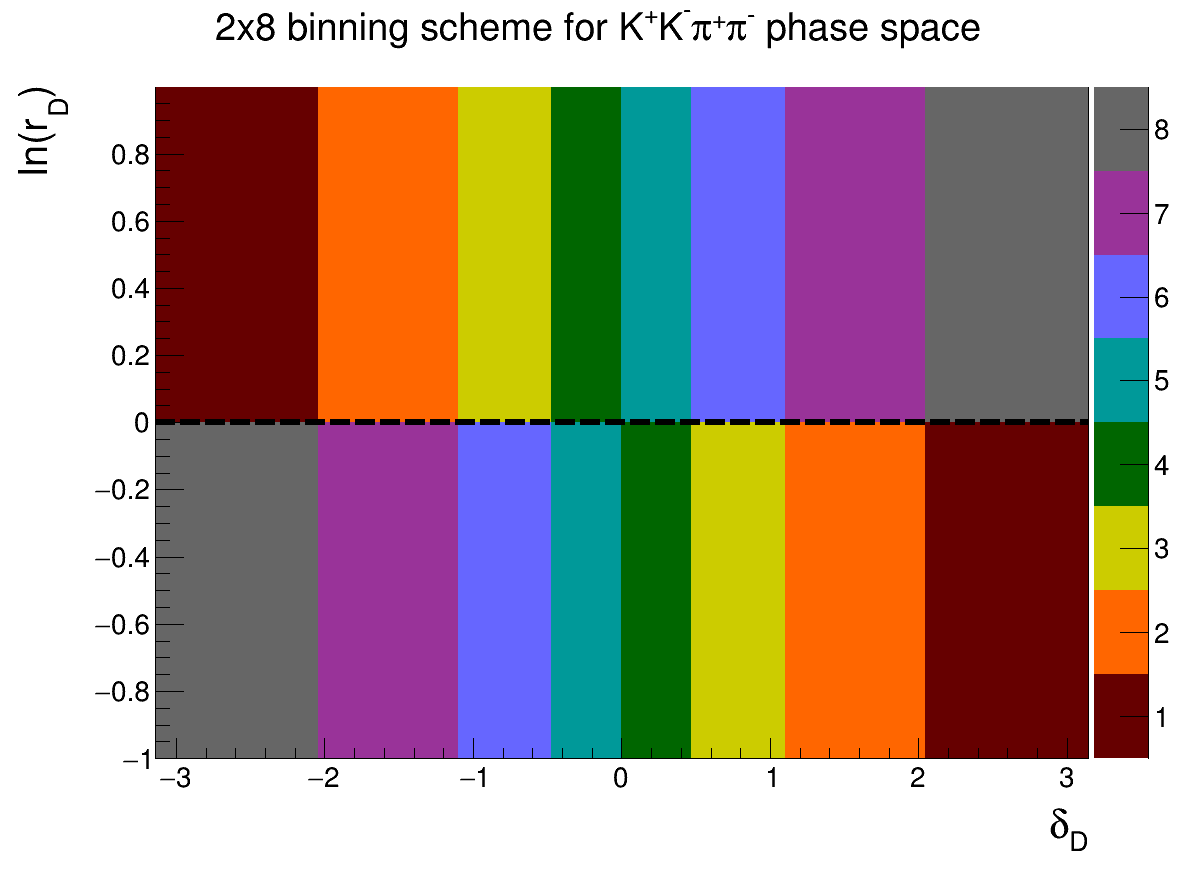
\includegraphics[width = 0.7\textwidth]{Plots/BinningSchemePlot_8Bins.png}
  \end{figure}
  \vspace{-1.0cm}
  \begin{center}
    $Q = 0.90$ \\
    Bins $i < 0$ on top, $i > 0$ below
  \end{center}
\end{frame}

\begin{frame}{$\gamma$ precision benchmark}
  \begin{itemize}
    \item{Generate $2000$ $B^\pm\to DK^\pm$ candidates using LHCb model in AmpGen}
    \item{Fit back with same model using AmpGen}
  \end{itemize}
  \begin{figure}
    \centering
    \vspace{-0.2cm}
    \begin{subfigure}{0.5\textwidth}
      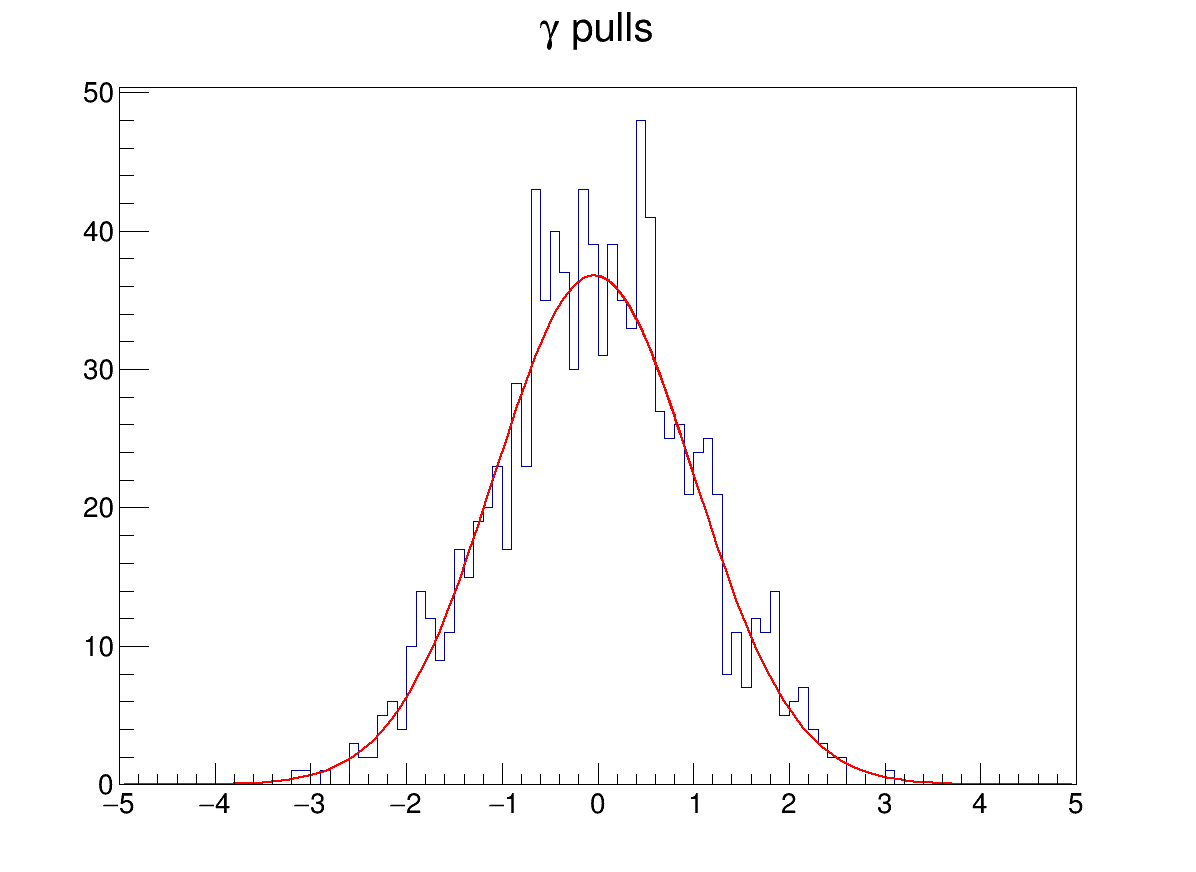
\includegraphics[width = 1.0\textwidth]{Plots/AmpGen_UnbinnedFit_gamma_pull.png}
      \caption{Pull of $\gamma$}
    \end{subfigure}%
    \begin{subfigure}{0.5\textwidth}
      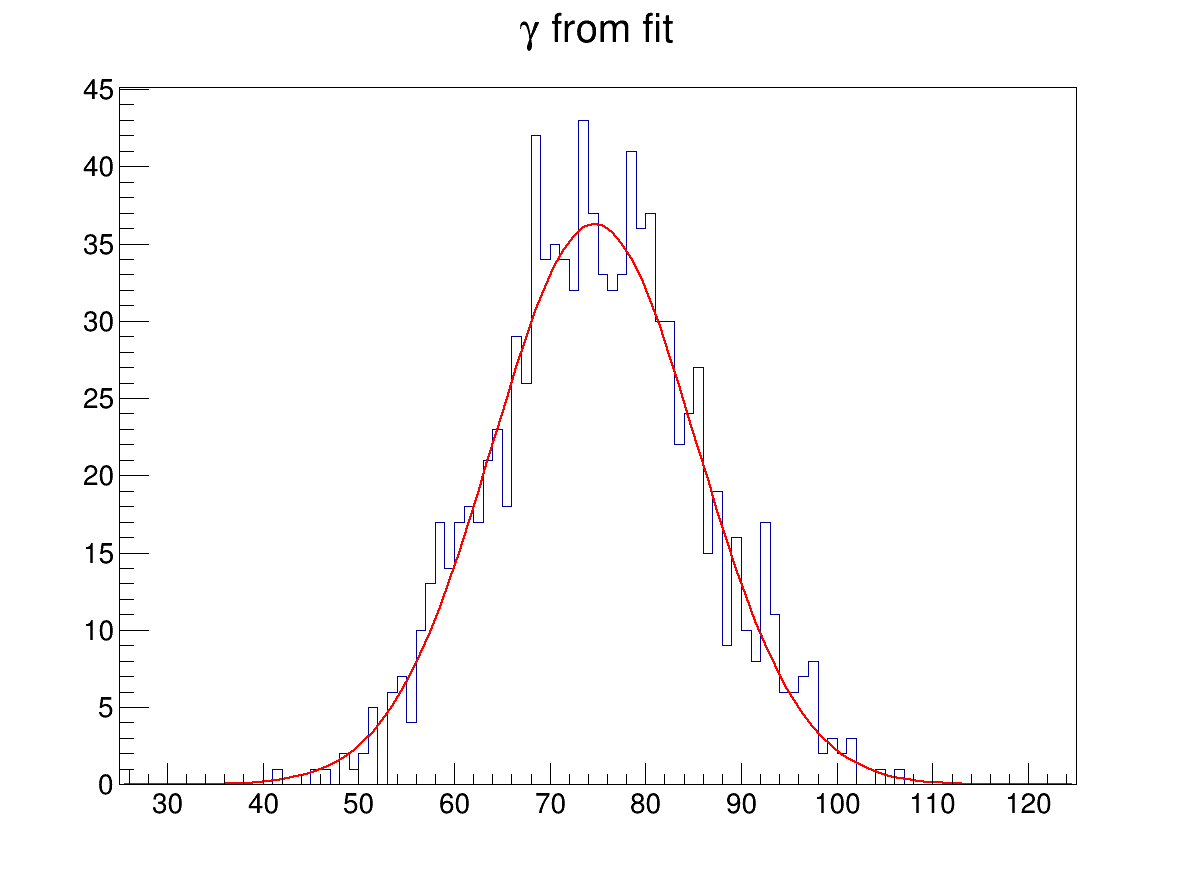
\includegraphics[width = 1.0\textwidth]{Plots/AmpGen_UnbinnedFit_gamma_fitted.png}
      \caption{Fitted $\gamma$ values}
    \end{subfigure}
  \end{figure}
  \begin{center}
    Precision of $\gamma$ in unbinned fit: $11^\circ$
  \end{center}
\end{frame}

\begin{frame}{Study of $\gamma$ precision}
  \begin{itemize}
    \item{Binned fit setup: Optimized $2\times 8$ bins}
    \item{Fit same AmpGen samples, using $c_i$, $s_i$ and $F_i$ from LHCb model}
  \end{itemize}
  \begin{figure}
    \centering
    \vspace{-0.2cm}
    \begin{subfigure}{0.5\textwidth}
      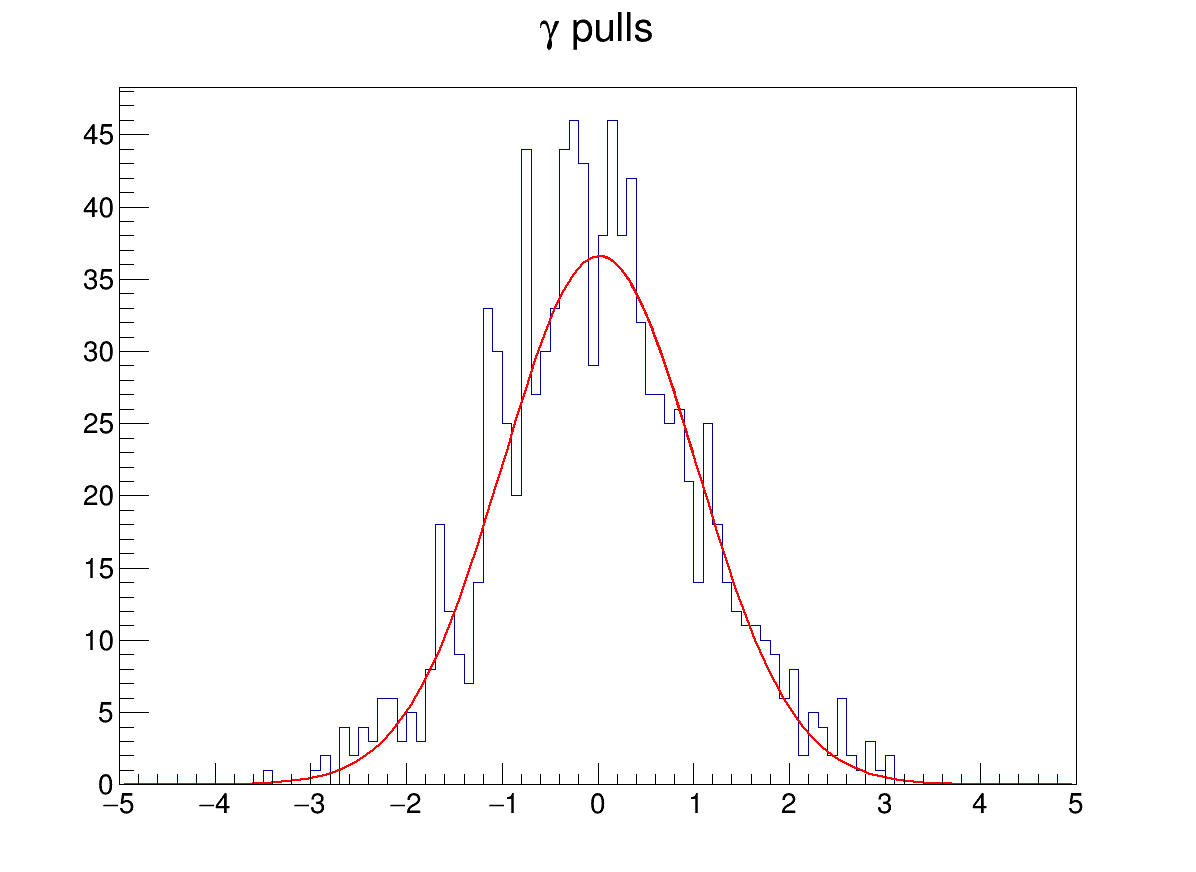
\includegraphics[width = 1.0\textwidth]{Plots/BinnedFit_gamma_pull.png}
      \caption{Pull of $\gamma$}
    \end{subfigure}%
    \begin{subfigure}{0.5\textwidth}
      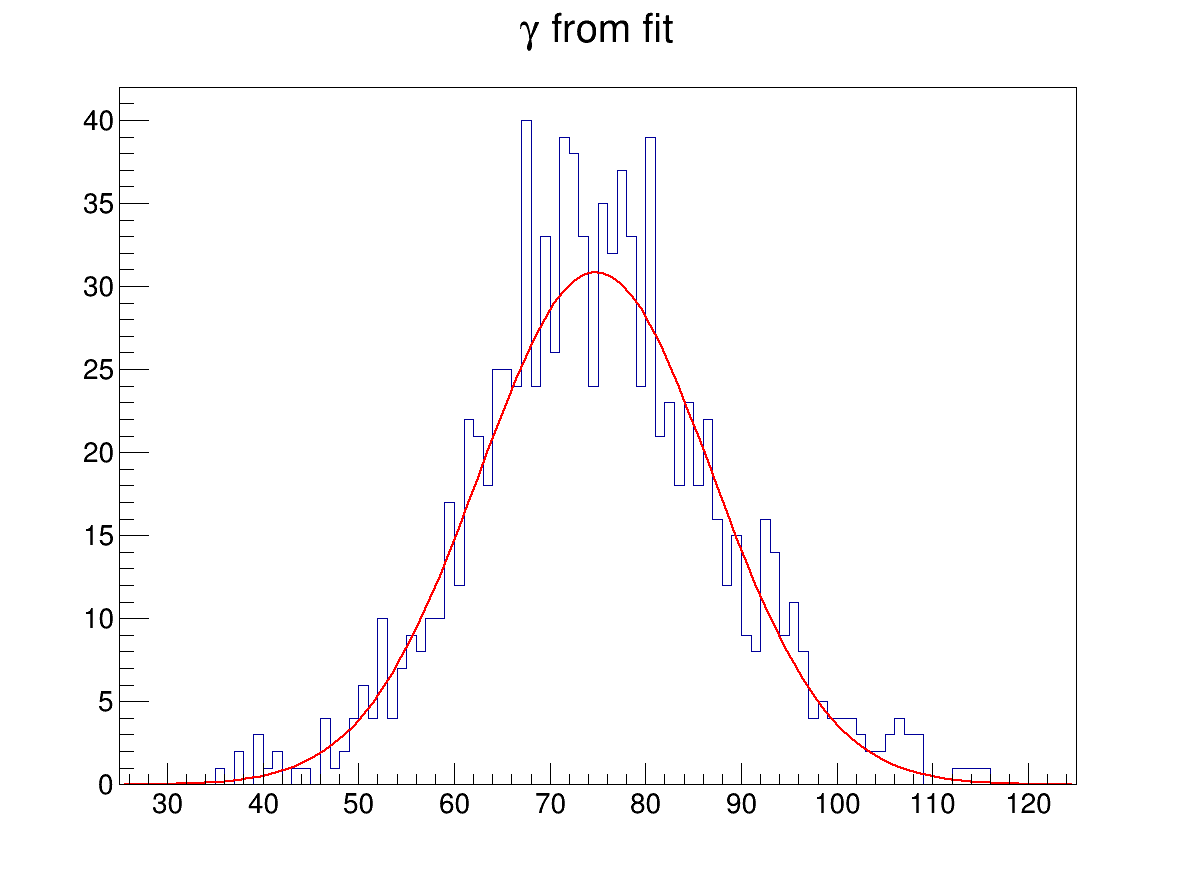
\includegraphics[width = 1.0\textwidth]{Plots/BinnedFit_gamma_fitted.png}
      \caption{Fitted $\gamma$ values}
    \end{subfigure}
  \end{figure}
  \begin{center}
    Precision of $\gamma$ in binned fit: $12^\circ$ \\
    Consistent with unbinned fit and $Q$-value
  \end{center}
\end{frame}

\section{\texorpdfstring{$B^\pm\to(K^+K^-\pi^+\pi^-)_Dh^\pm$}{B to K+ K- pi+ pi- h} selection}
\begin{frame}{$B^\pm\to(K^+K^-\pi^+\pi^-)_Dh^\pm$ selection}
  \begin{center}
    {\huge $B^\pm\to(K^+K^-\pi^+\pi^-)_Dh^\pm$ selection}
  \end{center}
\end{frame}

\begin{frame}{Samples}
  \begin{itemize}
    \setlength\itemsep{1.2em}
    \item{Data sample: Full Run 1 and 2}
    \item{MC samples: Full Run 1 and 2 excluding 2015}
    \begin{itemize}
      \item{AmpGen model}
      \item{Large filtered samples}
    \end{itemize}
  \end{itemize}
  \begin{block}{Stripping lines}
    $\text{StrippingB2D0PiD2HHHHBeauty2CharmLineDecision}$ \\
    $\text{StrippingB2D0KD2HHHHBeauty2CharmLineDecision}$
  \end{block}
\end{frame}

\begin{frame}{Boosted Decision Tree}
  \begin{itemize}
    \setlength\itemsep{1.2em}
    \item{BDTG from TMVA Toolkit}
    \item{Signal sample: $B^\pm\to DK^\pm$ and $B^\pm\to D\pi^\pm$ MC samples}
    \item{Background sample: Data sample with $m_{B^\pm}^\text{DTF}\in[5800, 7000]\si{\mega\eV}$}
    \item{Random, equal sized test and training samples}
  \end{itemize}
\end{frame}

\begin{frame}{BDT training results}
  \begin{figure}
    \centering
    \vspace{-0.2cm}
    \begin{subfigure}{0.5\textwidth}
      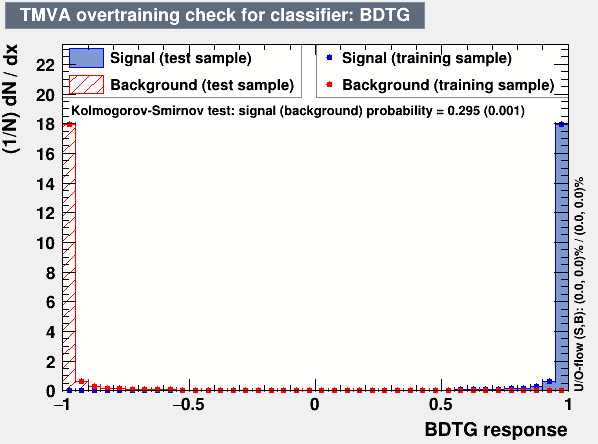
\includegraphics[width = 1.0\textwidth]{Plots/overtrain_BDTG.png}
      \caption{BDT output}
    \end{subfigure}%
    \begin{subfigure}{0.5\textwidth}
      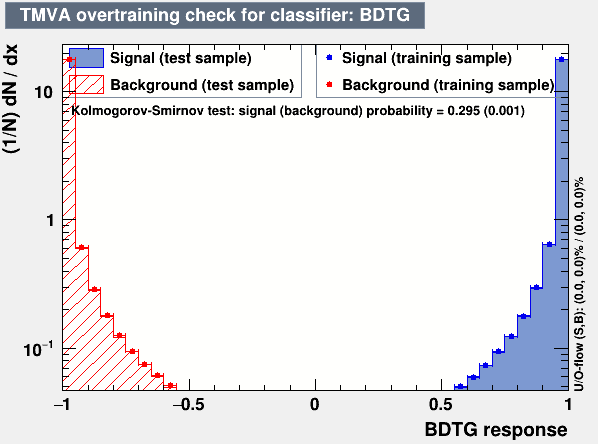
\includegraphics[width = 1.0\textwidth]{Plots/overtrain_BDTG_log.png}
      \caption{BDT output on a logarithmic scale}
    \end{subfigure}
  \end{figure}
\end{frame}

\begin{frame}{BDT optimization study}
  \begin{figure}
    \centering
    \vspace{-0.2cm}
    \begin{subfigure}{0.5\textwidth}
      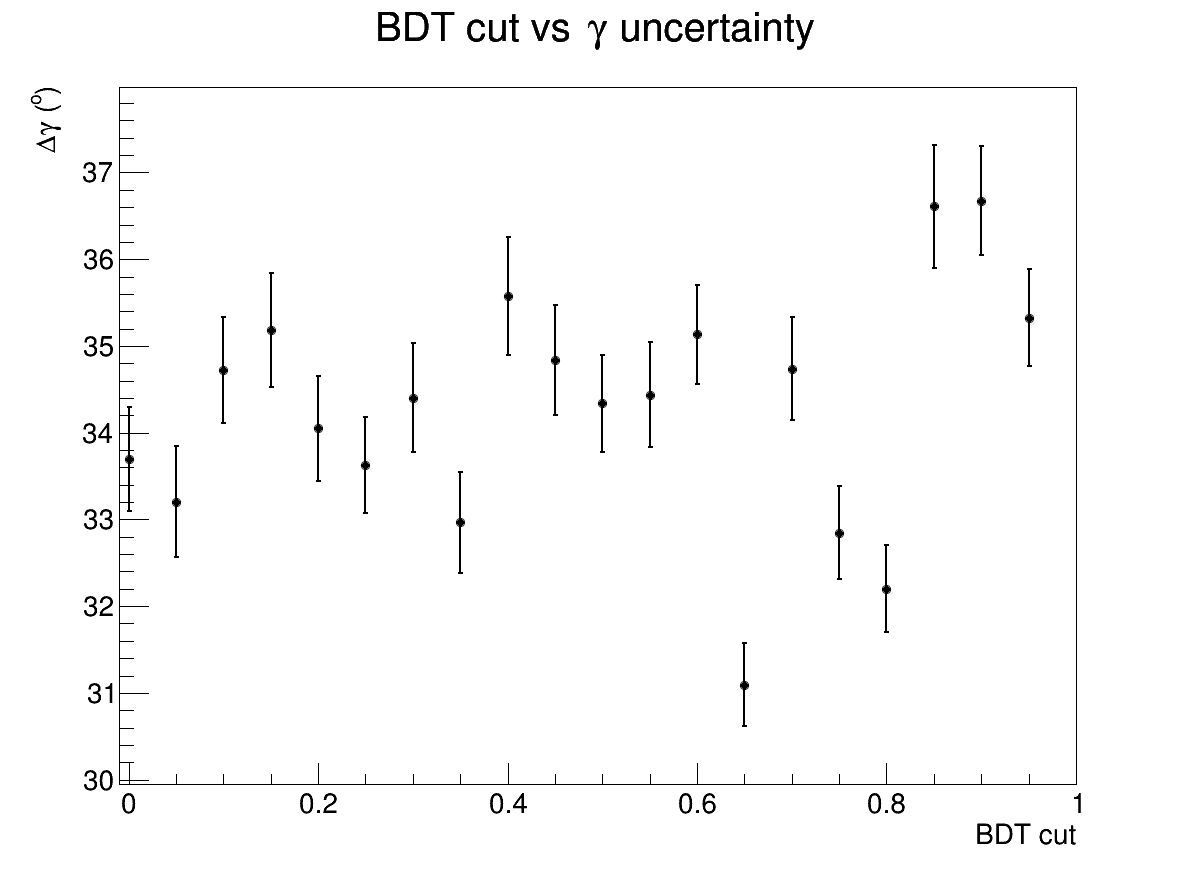
\includegraphics[width = 1.0\textwidth]{Plots/BDTCutVersusGammaErrorRun1.png}
      \caption{Run $1$}
    \end{subfigure}%
    \begin{subfigure}{0.5\textwidth}
      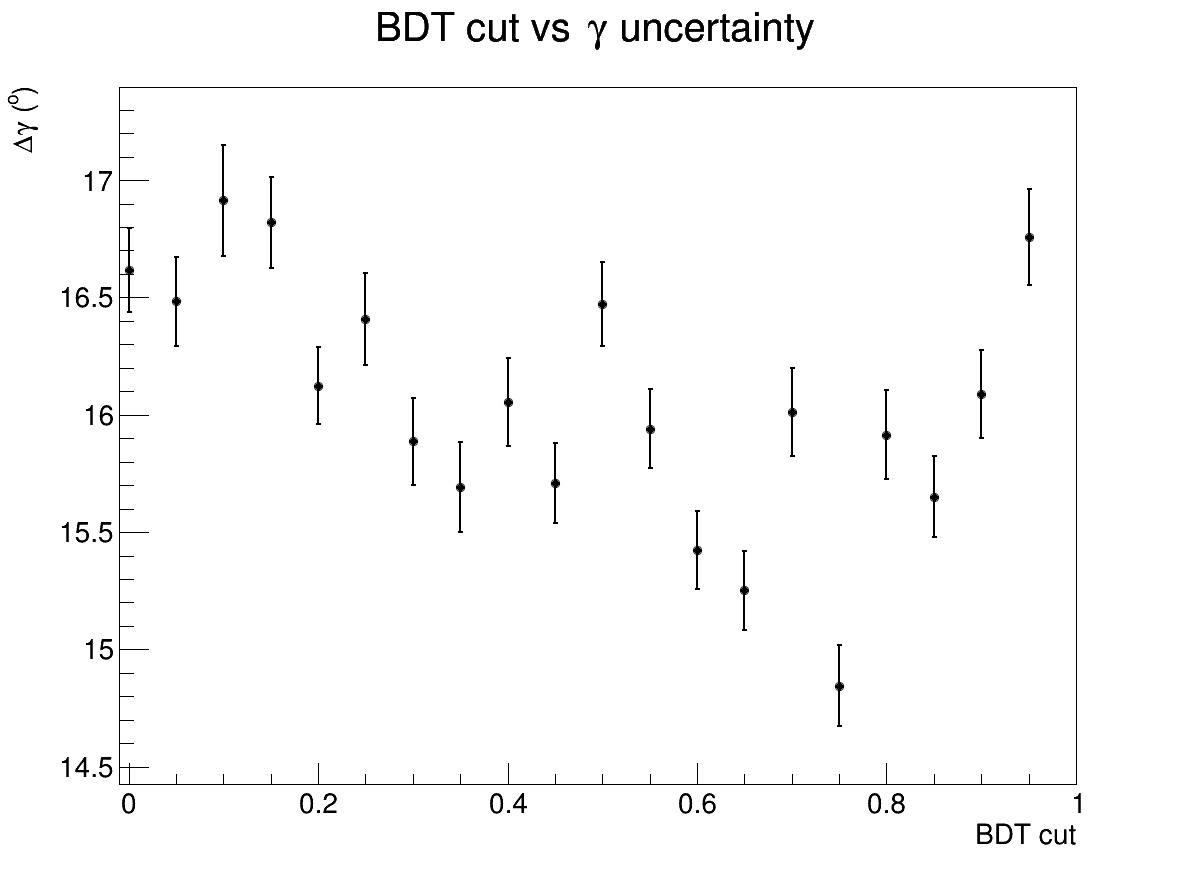
\includegraphics[width = 1.0\textwidth]{Plots/BDTCutVersusGammaErrorRun2.png}
      \caption{Run $2$}
    \end{subfigure}
  \end{figure}
  \begin{itemize}
    \item{Run $1$: Pick BDT working point at 0.65}
    \item{Run $2$: Pick BDT working point at 0.75}
  \end{itemize}
\end{frame}

\section{Backgrounds}
\begin{frame}{Backgrounds}
  \begin{center}
    {\huge Backgrounds}
  \end{center}
\end{frame}

\begin{frame}{$D\to K\pi\pi\pi$ mis-ID background}
  \begin{itemize}
    \setlength\itemsep{0.5em}
    \item{$B^\pm\to Dh^\pm$, $D\to K\pi\pi\pi$}
    \item{Single mis-ID: $K\pi\pi\pi\to KK\pi\pi$}
    \item{Triple mis-ID: $\pi\pi K\pi\to KK\pi\pi$}
    \item{Use LHCb MC generated with AmpGen, reweight with PIDCalib2}
  \end{itemize}
  \begin{figure}
    \centering
    \begin{subfigure}{0.45\textwidth}
      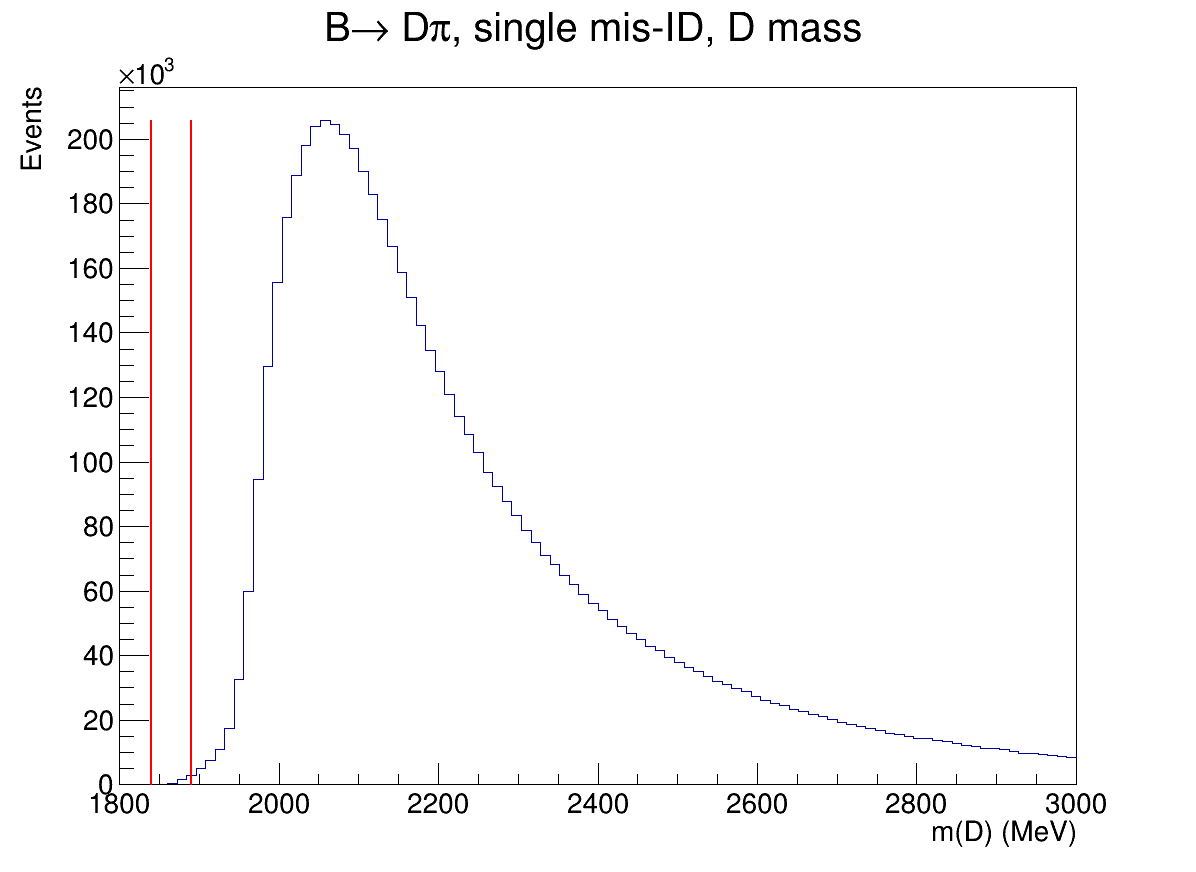
\includegraphics[width = 1.0\textwidth]{Plots/Kpipipi_SingleMisID_Dpi_DMass.png}
      \caption{Single mis-ID}
    \end{subfigure}%
    \begin{subfigure}{0.45\textwidth}
      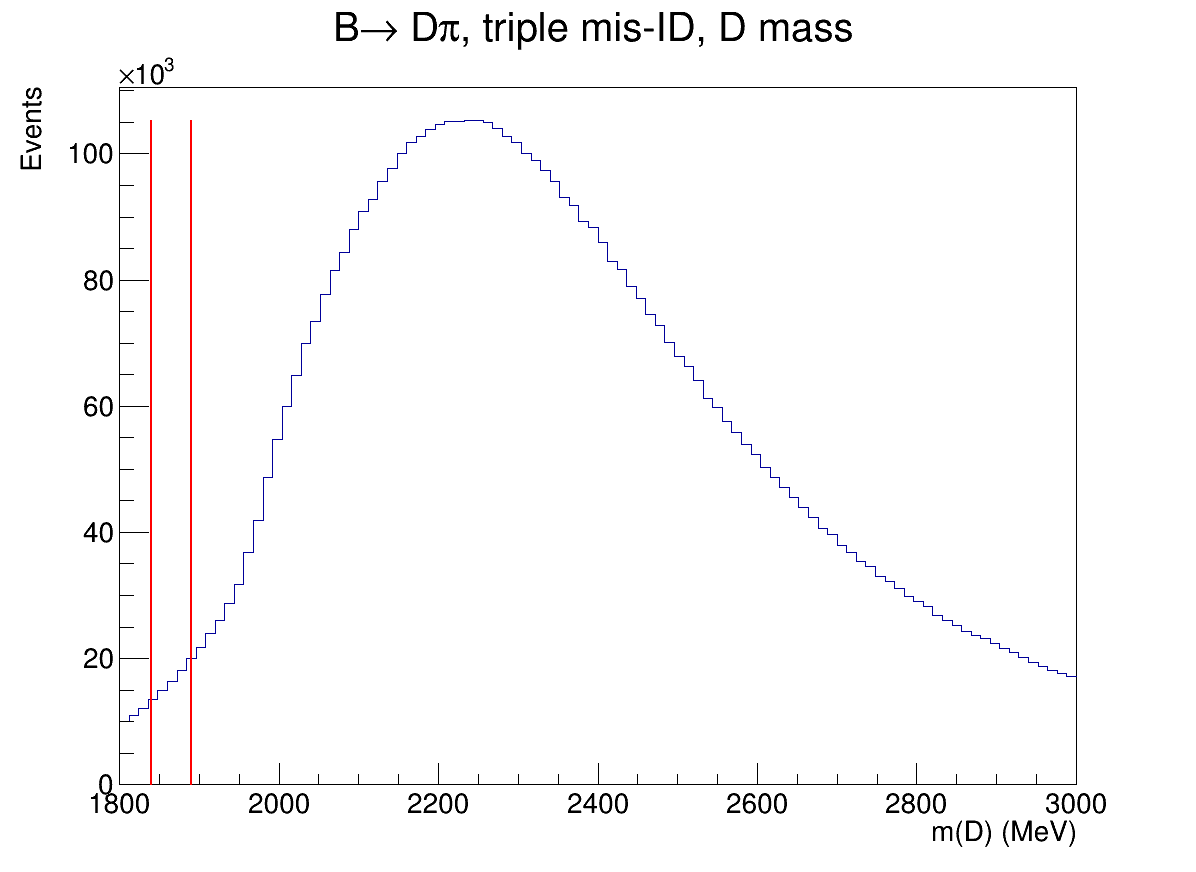
\includegraphics[width = 1.0\textwidth]{Plots/Kpipipi_TripleMisID_Dpi_DMass.png}
      \caption{Triple misID}
    \end{subfigure}
    \caption{$D$ invariant mass}
  \end{figure}
\end{frame}

\begin{frame}{$D\to K\pi\pi\pi$ mis-ID background}
  \begin{figure}
    \centering
    \begin{subfigure}{0.5\textwidth}
      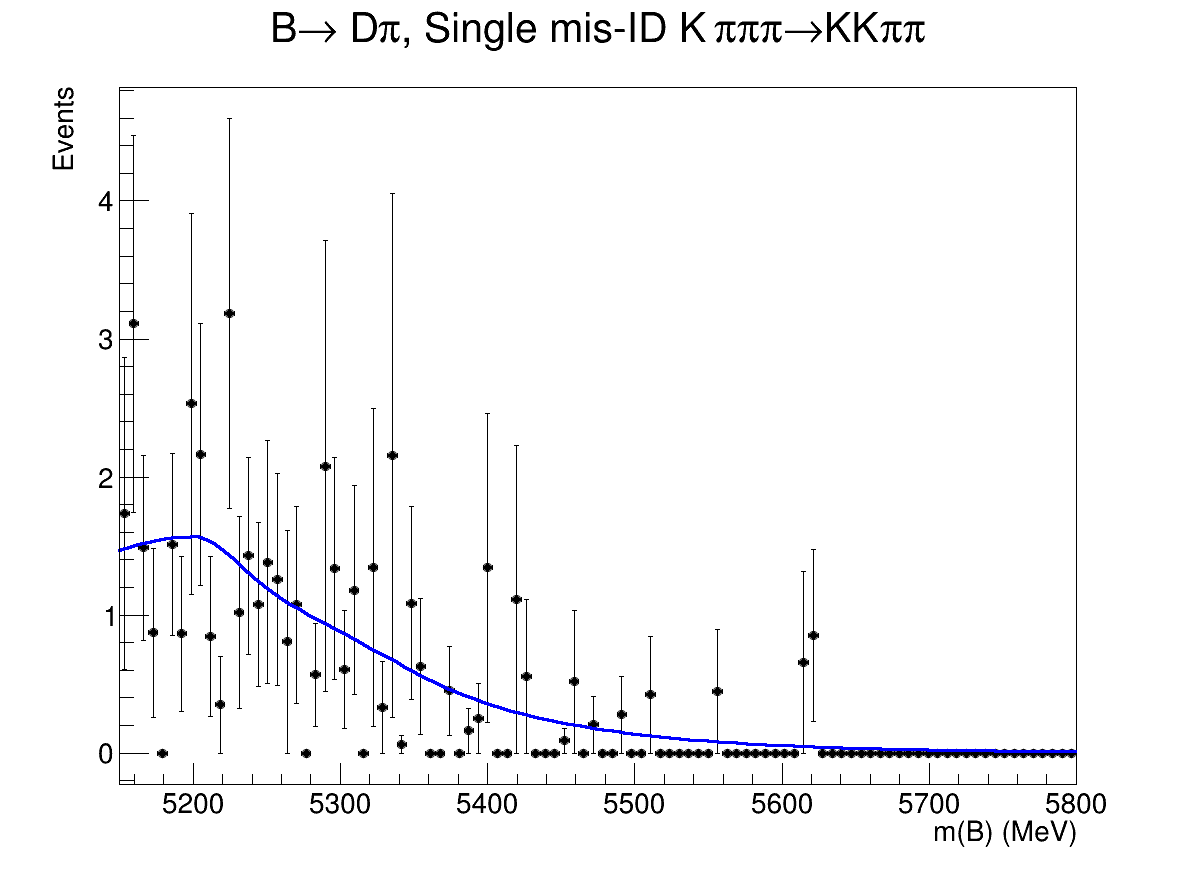
\includegraphics[width = 1.0\textwidth]{Plots/Kpipipi_SingleMisID_Dpi_BMass.png}
      \caption{Single mis-ID}
    \end{subfigure}%
    \begin{subfigure}{0.5\textwidth}
      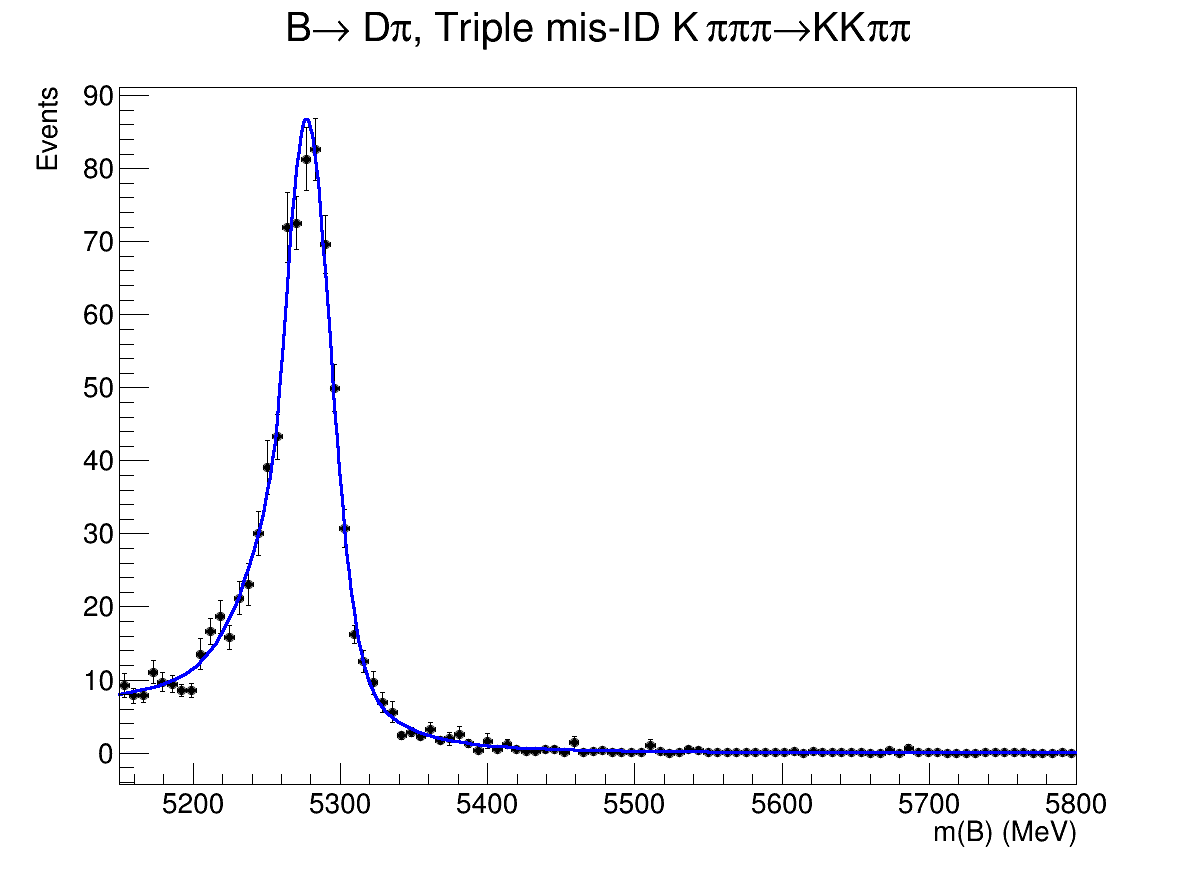
\includegraphics[width = 1.0\textwidth]{Plots/Kpipipi_TripleMisID_Dpi_BMass.png}
      \caption{Triple misID}
    \end{subfigure}
    \caption{$B$ invariant mass}
  \end{figure}
  \begin{center}
    Conclusion: Negligible impact, include in systematics
  \end{center}
\end{frame}

\begin{frame}{$D\to K\pi\pi\pi\pi^0$ mis-ID background}
  \begin{itemize}
    \setlength\itemsep{0.5em}
    \item{$B^\pm\to Dh^\pm$, $D\to K\pi\pi\pi[\pi^0]$}
    \item{$\pi^0$ not reconstructed $\to$ Lower $D$ mass}
    \item{Single mis-ID: $K\pi\pi\pi\to KK\pi\pi$ $\to$ Higher $D$ mass}
    \item{Generate RapidSim samples, reweight with PIDCalib2}
  \end{itemize}
  \begin{figure}
    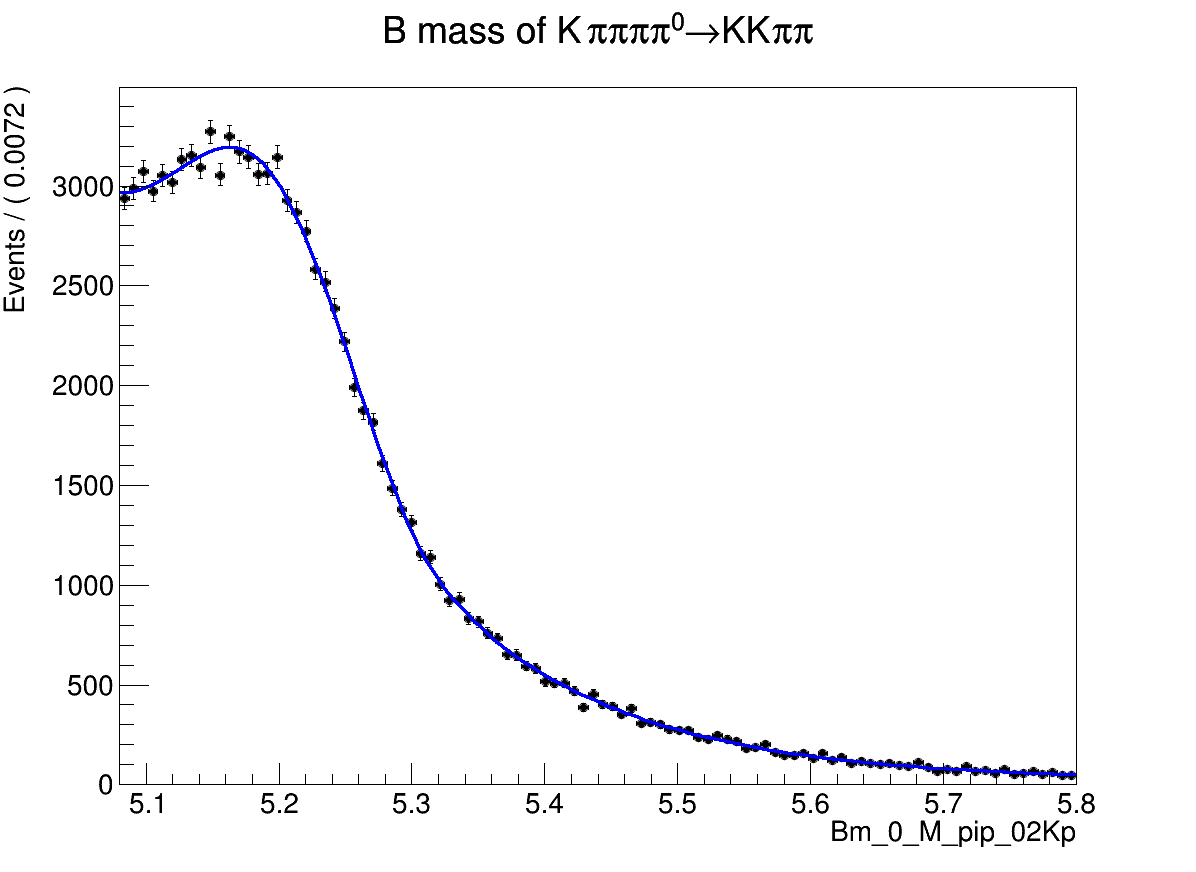
\includegraphics[width = 0.5\textwidth]{Plots/Kpipipipi0BMassB2DpiD2Kpipipi.png}
  \end{figure}
  \begin{center}
    Conclusion: Fix shape from RapidSim, allow yield to float
  \end{center}
\end{frame}

\section{Fit to data}
\begin{frame}{Global fit}
  \begin{center}
    {\huge Global fit}
  \end{center}
\end{frame}

\begin{frame}{Signal parameterisation}
  \begin{itemize}
    \setlength\itemsep{1.2em}
    \item{PDF shape parameterization identical to LHCb-ANA-2020-001}
    \item{Signal: Gaussian + Modified Cruijff}
    \item{Shape fixed from MC, yield and width floated}
    \item{Exponential background}
  \end{itemize}
  \vspace{0.5cm}
  \begin{equation*}
    f_\text{MG}(m|m_B, \sigma, \alpha_L, \alpha_R, \beta)\propto
    \begin{cases}
      \exp\Big(\frac{-\Delta m^2(1 + \beta\Delta m^2)}{2\sigma^2 + \alpha_L\Delta m^2}\Big), \quad \Delta m = m - m_B < 0 \\
      \exp\Big(\frac{-\Delta m^2(1 + \beta\Delta m^2)}{2\sigma^2 + \alpha_R\Delta m^2}\Big), \quad \Delta m = m - m_B > 0 \\
    \end{cases}
  \end{equation*}
\end{frame}

\begin{frame}{Partially reconstructed background}
  \begin{itemize}
    \setlength\itemsep{1.3em}
    \item{$B^\pm\to D\pi^\pm$:}
    \begin{enumerate}
    \setlength\itemsep{0.4em}
      \item{$B^\pm\to (D^{*0}\to D^0[\pi^0])\pi^\pm$}
      \item{$B^0\to (D^{*\mp}\to D^0[\pi^\mp])\pi^\pm$}
      \item{$B^{\pm(0)}\to D^0[\pi^{0(\mp)}]\pi^\pm$}
      \item{$B^\pm\to(D^{*0}\to D^0[\gamma])\pi^\pm$}
    \end{enumerate}
    \item{$B^\pm\to DK^\pm$:}
    \begin{enumerate}
      \setlength\itemsep{0.4em}
      \item{$B^\pm\to (D^{*0}\to D^0[\pi^0])K^\pm$}
      \item{$B^0\to (D^{*\mp}\to D^0[\pi^\mp])K^\pm$}
      \item{$B^{\pm(0)}\to D^0[\pi^{0(\mp)}]K^\pm$}
      \item{$B^\pm\to(D^{*0}\to D^0[\gamma])K^\pm$}
      \item{$B_s^0\to\bar{D^0}[\pi^+]K^-$}
      \item{Mis-ID from partially reconstructed $B^\pm\to D\pi^\pm$ channel}
    \end{enumerate}
  \end{itemize}
\end{frame}

\begin{frame}{Global fit}
  \begin{figure}
    \centering
    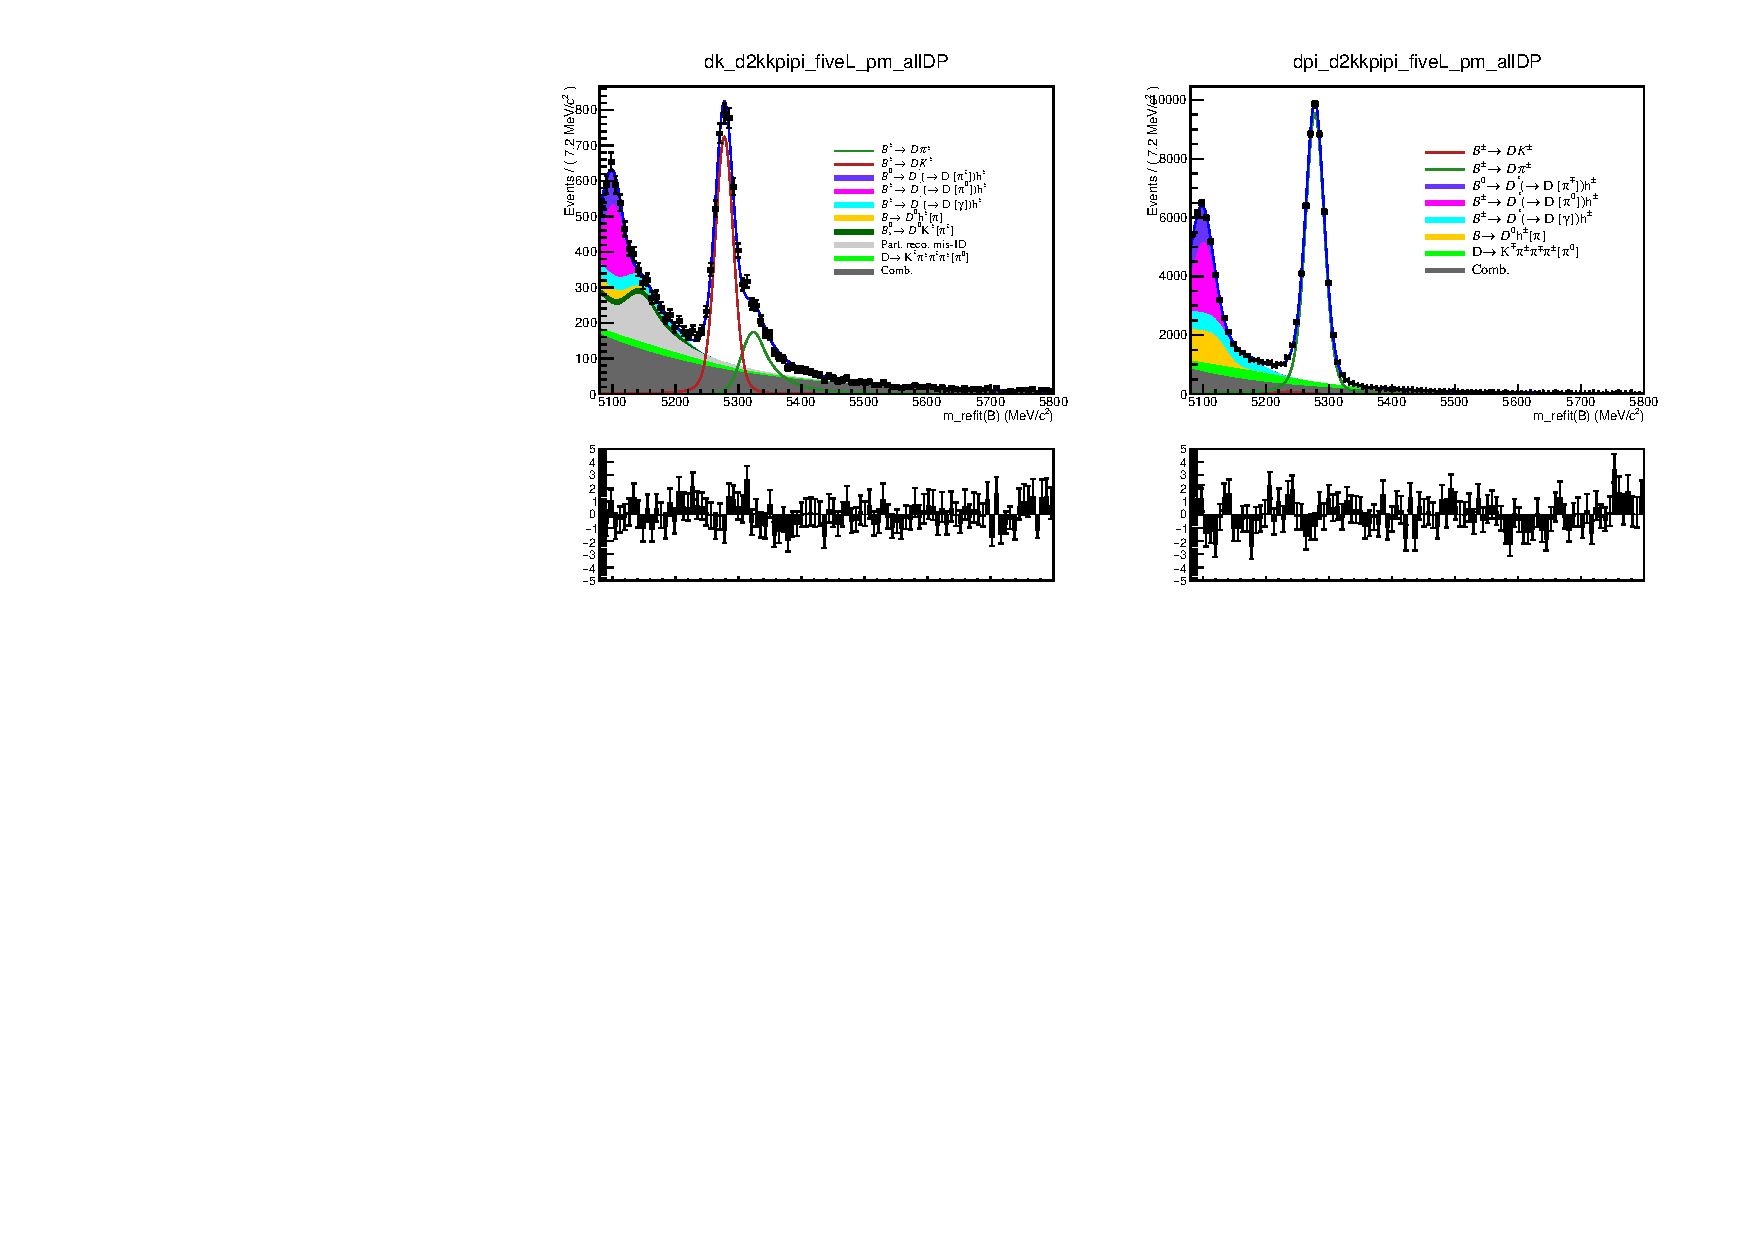
\includegraphics[width = 1.0\textwidth]{Plots/d2kkpipi_fiveL_allDP.pdf}
    \caption{$B^\pm\to DK^\pm$ channel (left) and $B^\pm\to D\pi^\pm$ channel (right)}
  \end{figure}
  \vspace{-0.5cm}
  \begin{itemize}
    \item{$B^\pm\to DK^\pm$ yield: $\SI{3543(75)}{}$}
    \item{$B^\pm\to D\pi^\pm$ yield: $\SI{47503(260)}{}$}
  \end{itemize}
\end{frame}

\begin{frame}{Binned CP fit}
  \begin{center}
    {\huge Binned CP fit}
  \end{center}
\end{frame}

\begin{frame}{Binned CP fit}
  \begin{itemize}
    \setlength\itemsep{1.2em}
    \item{Use $2\times 8$ bins}
    \item{$c_i$ and $s_i$ calculated using MC integration of LHCb amplitude model}
    \item{Fit for CP observables}
    \item{PDF shape parameters fixed from global fit}
    \item{Yield of signal, low mass partially reconstructed background and combinatorial background floated}
    \item{Fractional yields $F_i$ floated}
  \end{itemize}
  \begin{equation*}
    \mathcal{R}_i = 
    \begin{cases}
      F_i, \quad i = -8 \\
      F_i/\sum_{j\geq i}, -8 < i\leq+8
    \end{cases}
  \end{equation*}
\end{frame}

\begin{frame}{CP observables result: $x_-^{DK}$}
  \begin{figure}
    \centering
    \begin{subfigure}{0.42\textwidth}
      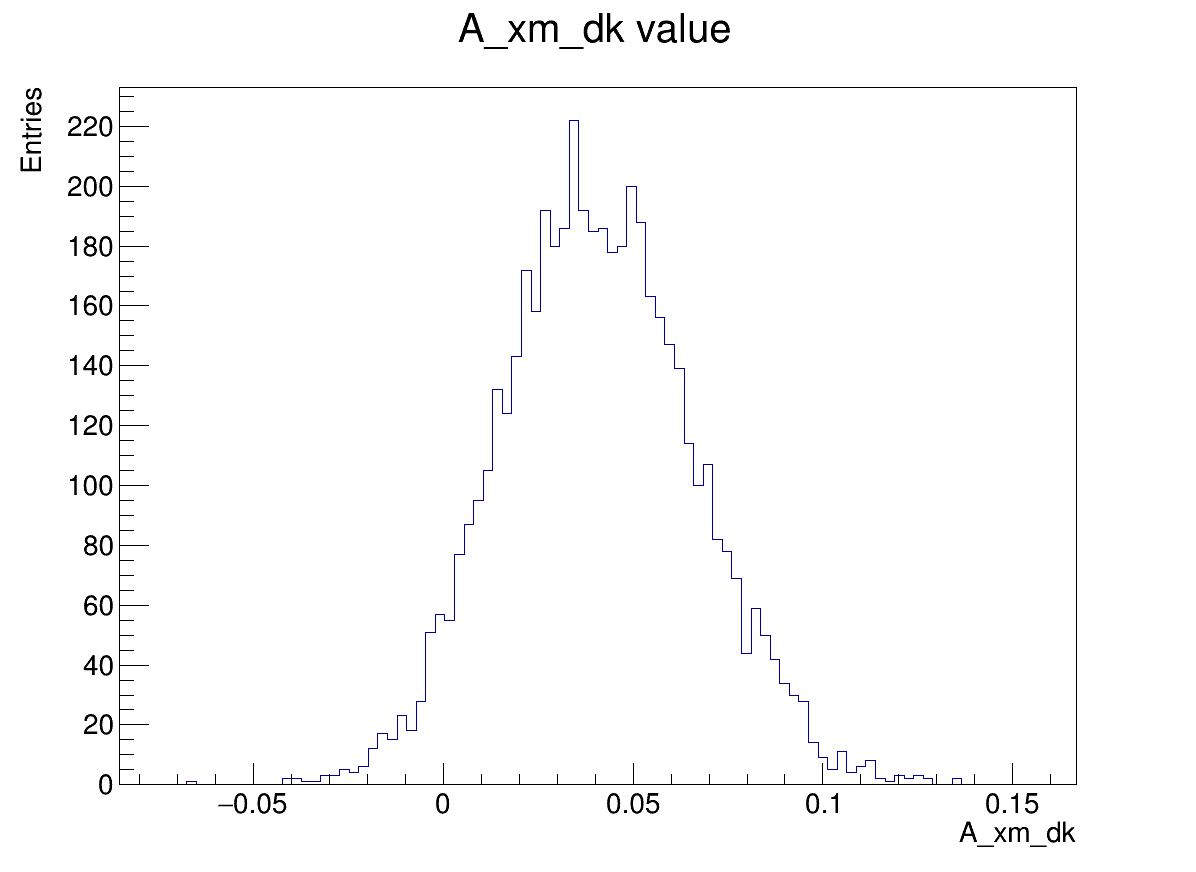
\includegraphics[width = 1.0\textwidth]{Plots/A_xm_dk_value.png}
    \end{subfigure}
    \begin{subfigure}{0.42\textwidth}
      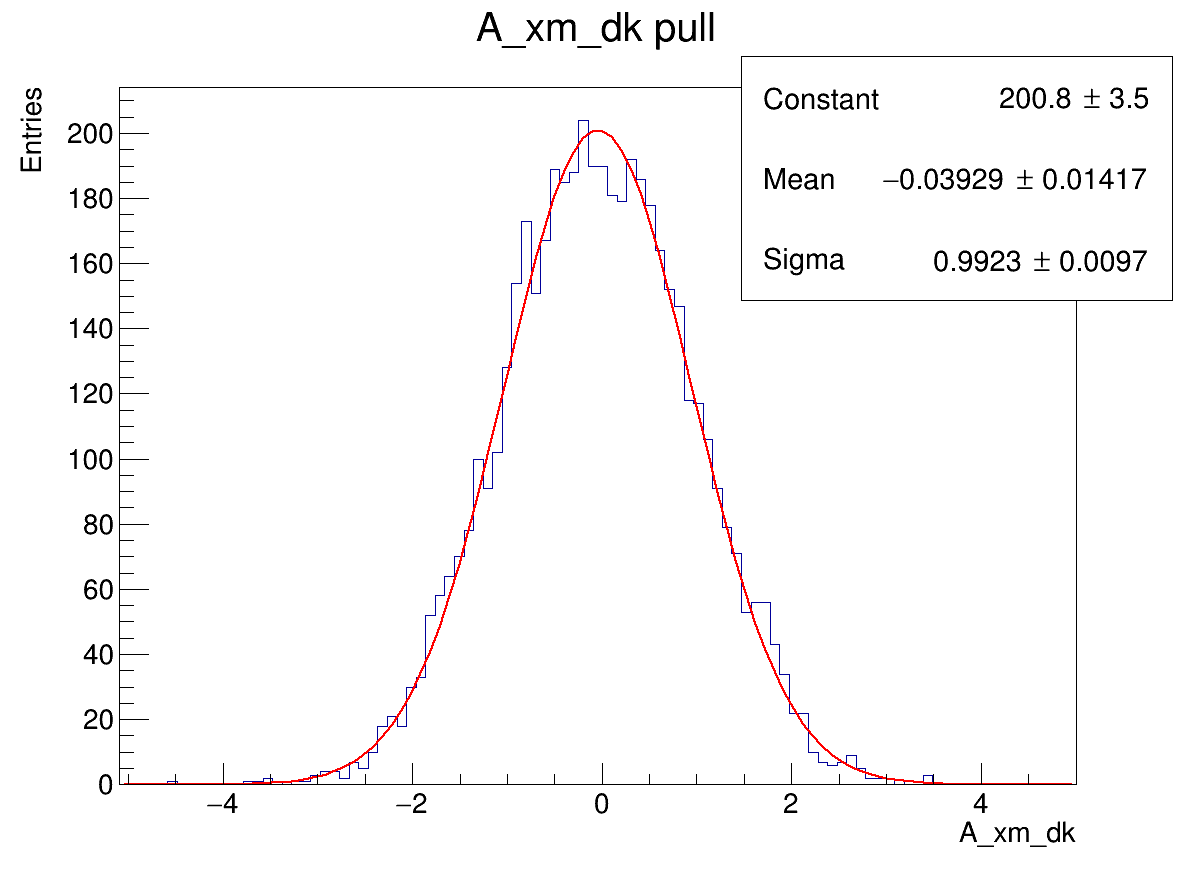
\includegraphics[width = 1.0\textwidth]{Plots/A_xm_dk_pull.png}
    \end{subfigure}%
    \begin{subfigure}{0.42\textwidth}
      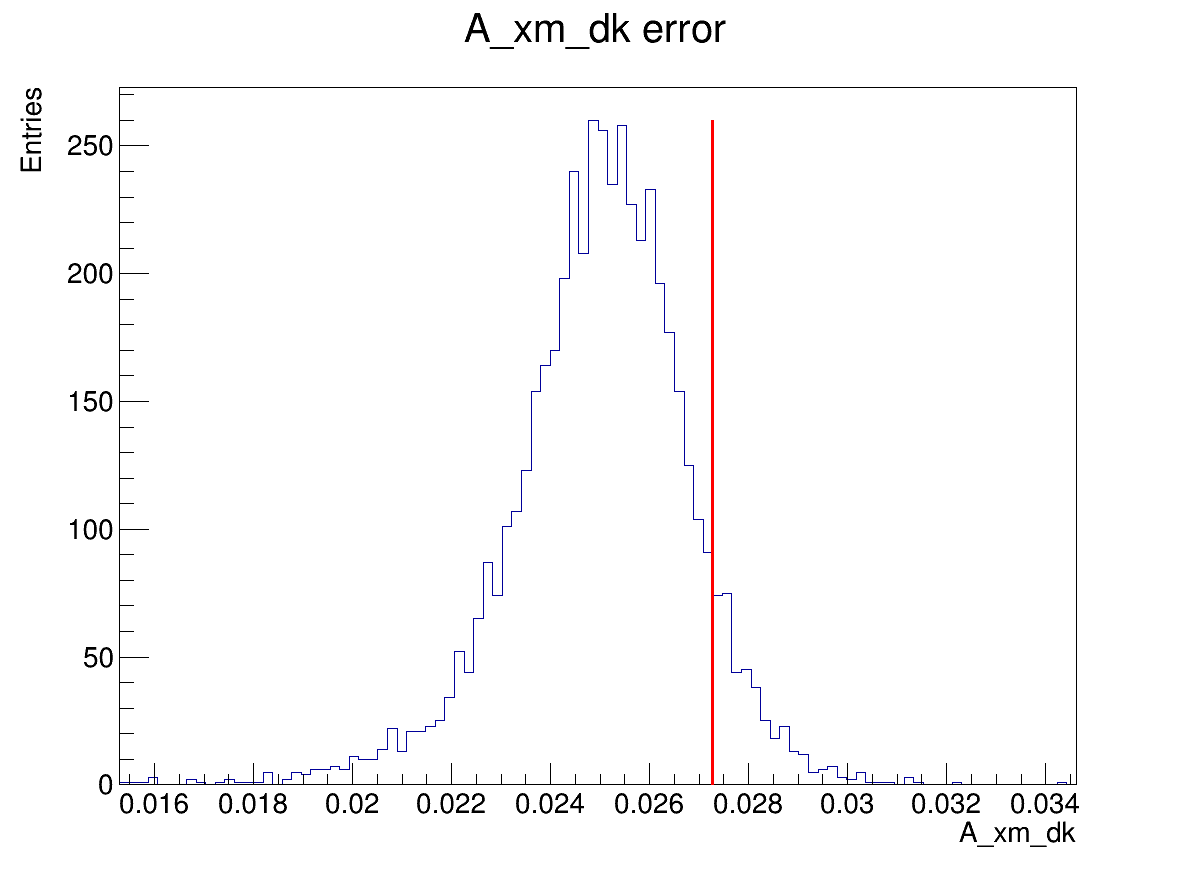
\includegraphics[width = 1.0\textwidth]{Plots/A_xm_dk_error_WithDataUncertainty.png}
    \end{subfigure}
  \end{figure}
\end{frame}

\begin{frame}{CP observables result: $y_-^{DK}$}
  \begin{figure}
    \centering
    \begin{subfigure}{0.42\textwidth}
      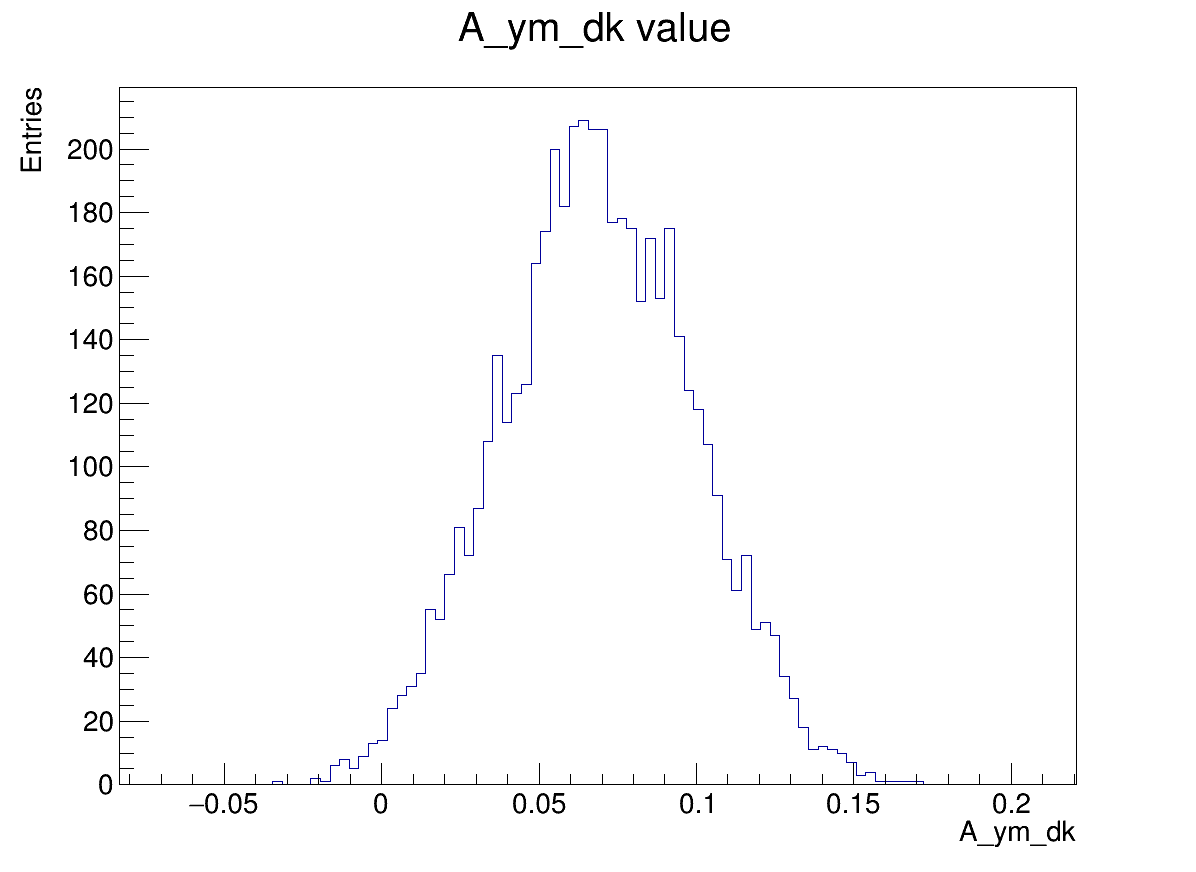
\includegraphics[width = 1.0\textwidth]{Plots/A_ym_dk_value.png}
    \end{subfigure}
    \begin{subfigure}{0.42\textwidth}
      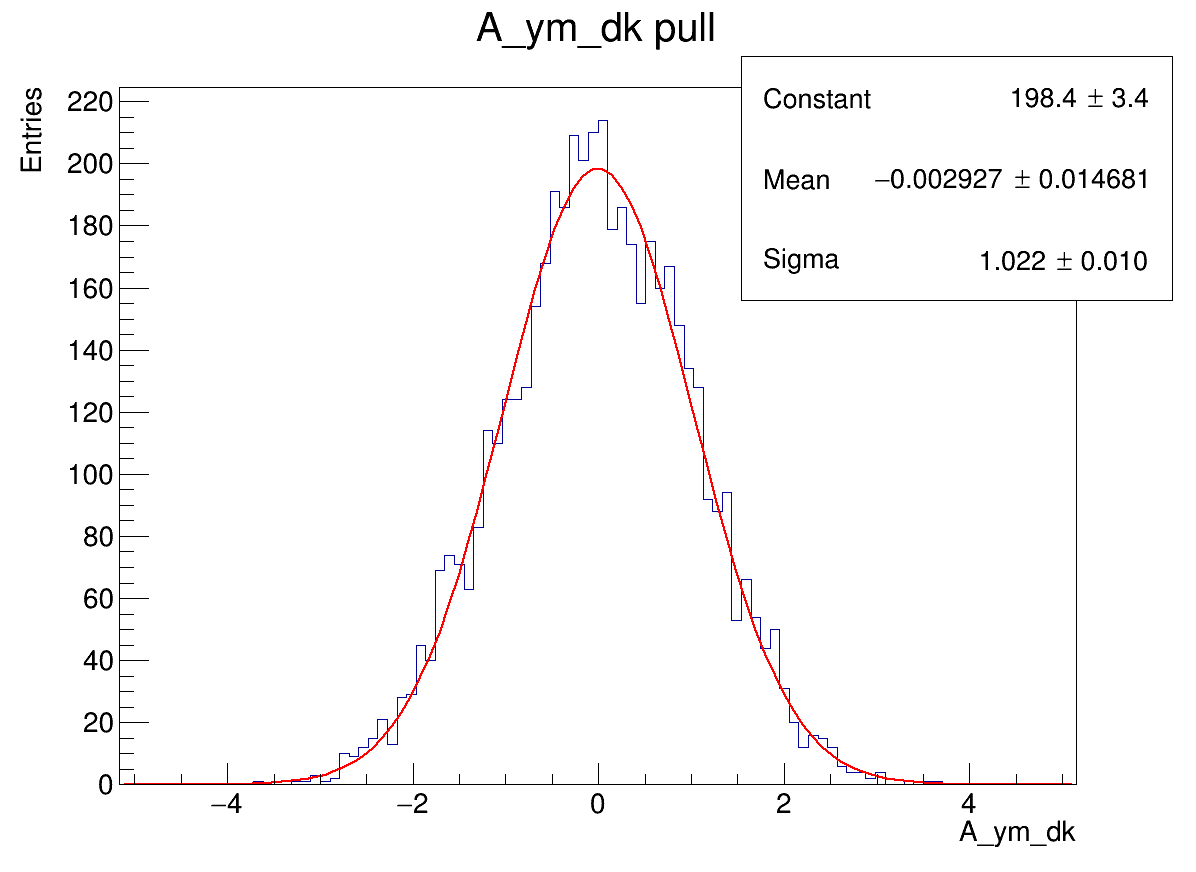
\includegraphics[width = 1.0\textwidth]{Plots/A_ym_dk_pull.png}
    \end{subfigure}%
    \begin{subfigure}{0.42\textwidth}
      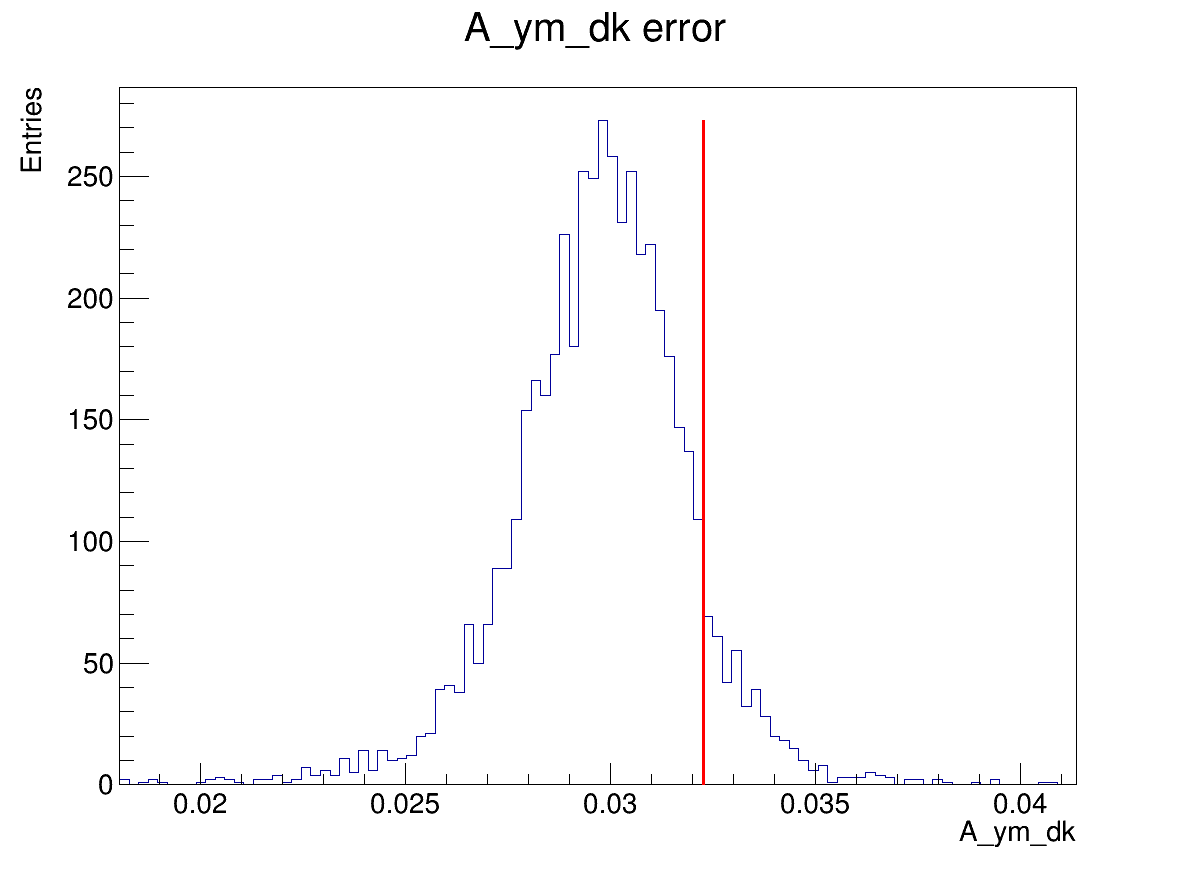
\includegraphics[width = 1.0\textwidth]{Plots/A_ym_dk_error_WithDataUncertainty.png}
    \end{subfigure}
  \end{figure}
\end{frame}

\begin{frame}{CP observables result: $x_+^{DK}$}
  \begin{figure}
    \centering
    \begin{subfigure}{0.42\textwidth}
      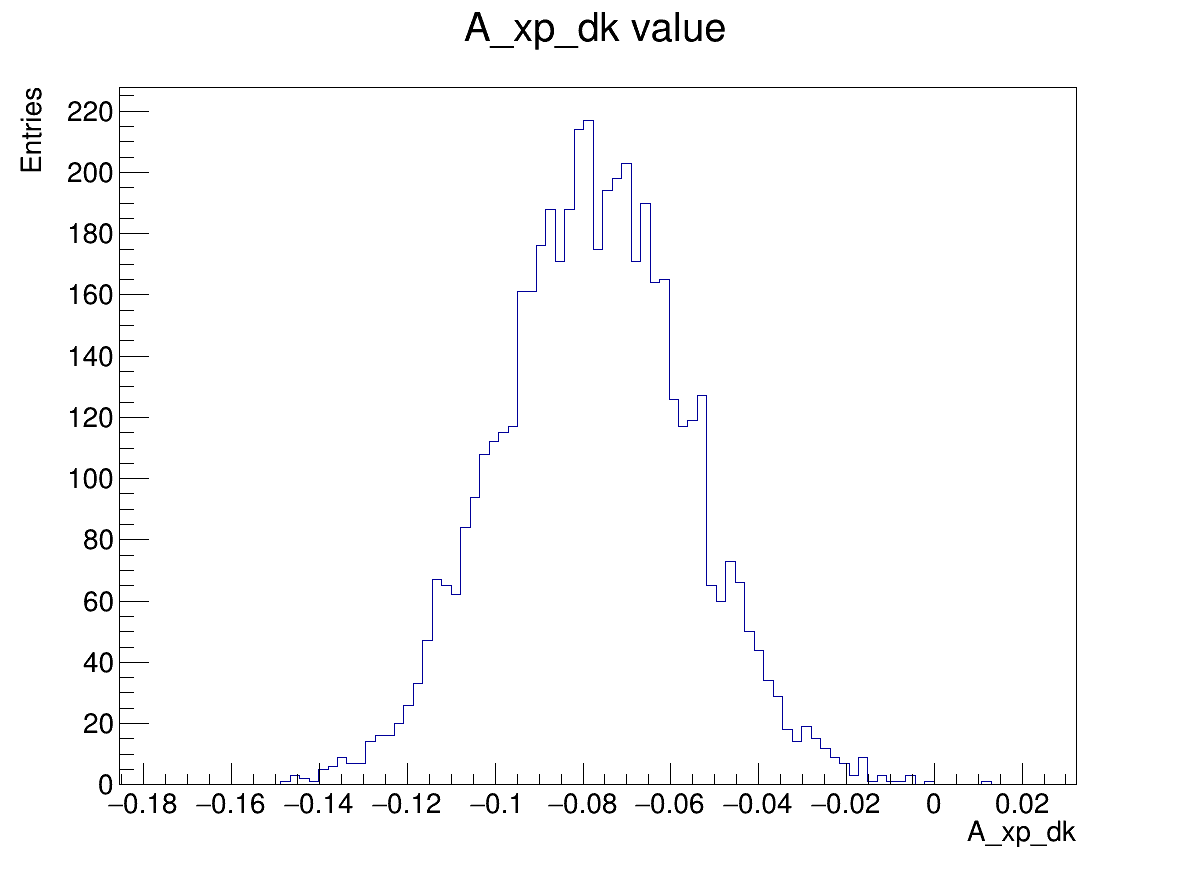
\includegraphics[width = 1.0\textwidth]{Plots/A_xp_dk_value.png}
    \end{subfigure}
    \begin{subfigure}{0.42\textwidth}
      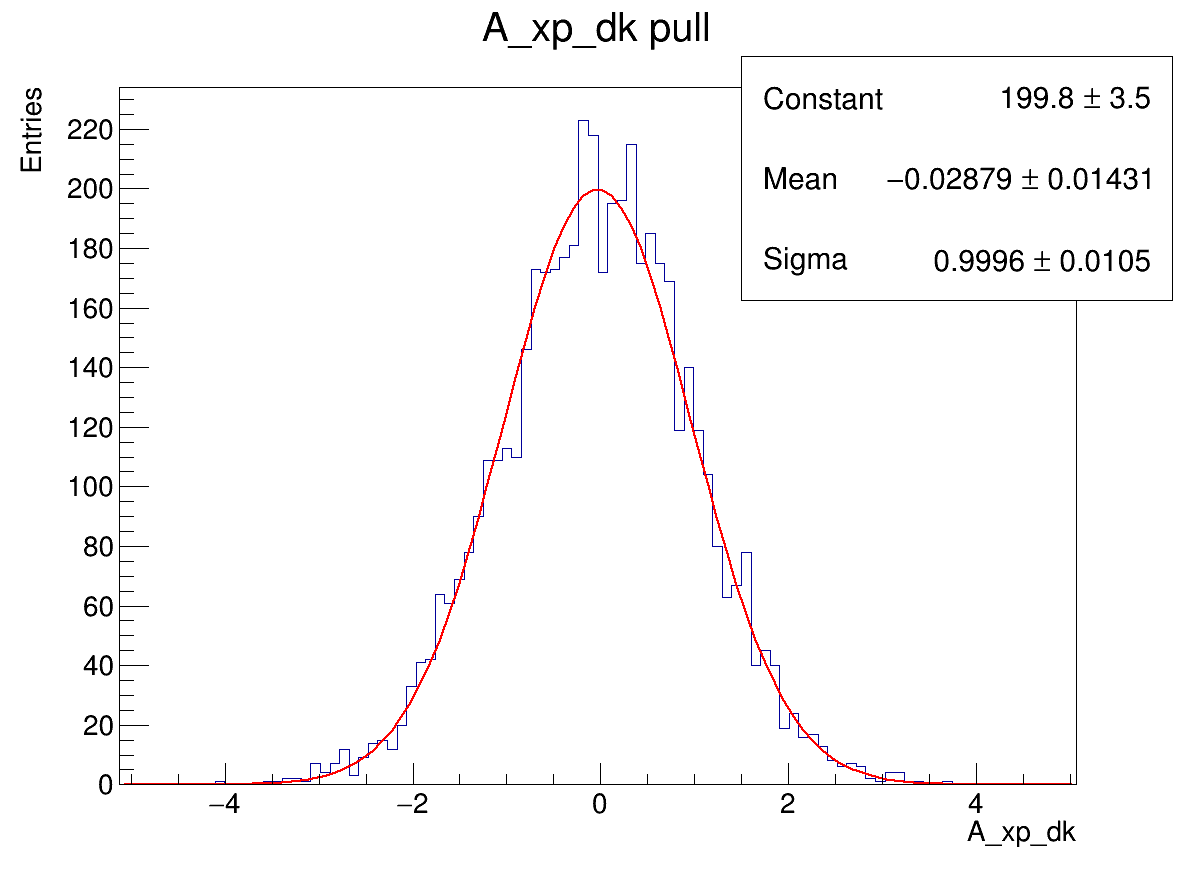
\includegraphics[width = 1.0\textwidth]{Plots/A_xp_dk_pull.png}
    \end{subfigure}%
    \begin{subfigure}{0.42\textwidth}
      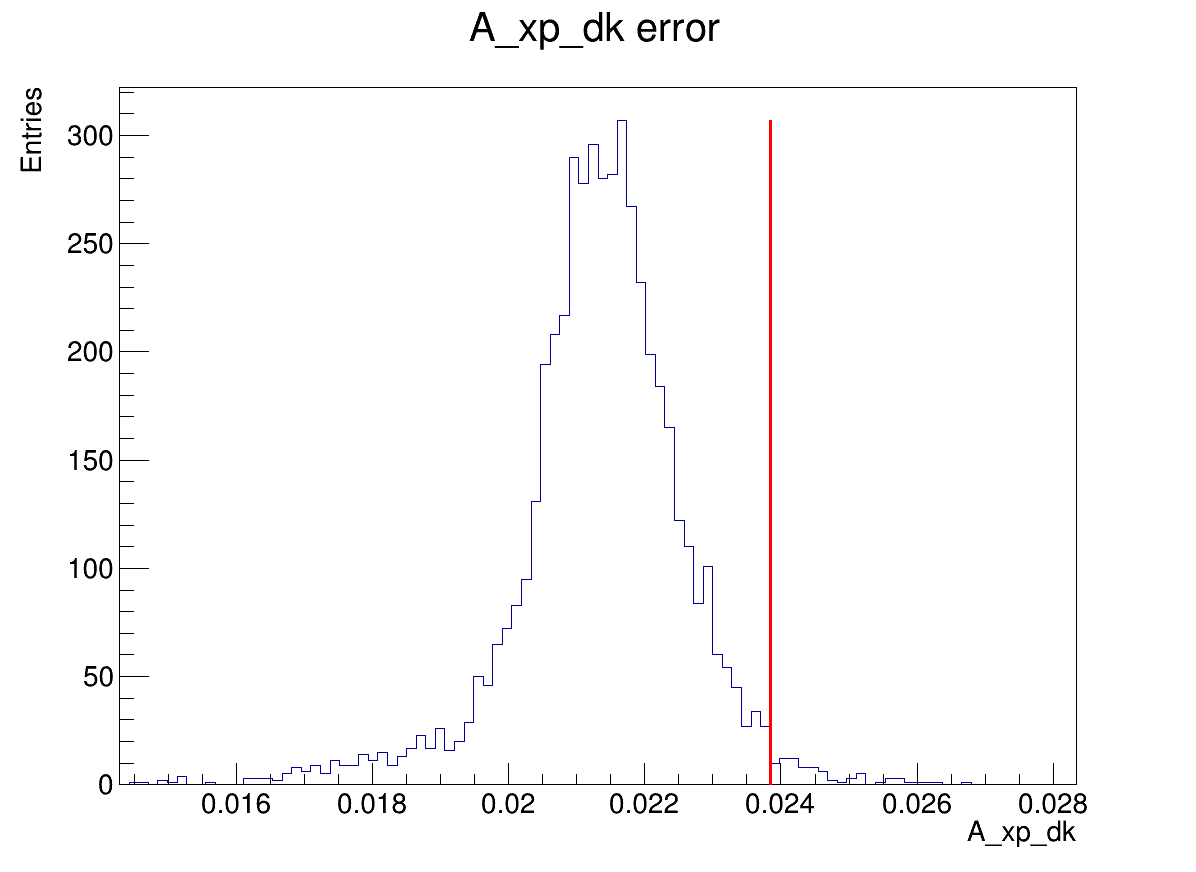
\includegraphics[width = 1.0\textwidth]{Plots/A_xp_dk_error_WithDataUncertainty.png}
    \end{subfigure}
  \end{figure}
\end{frame}

\begin{frame}{CP observables result: $y_+^{DK}$}
  \begin{figure}
    \centering
    \begin{subfigure}{0.42\textwidth}
      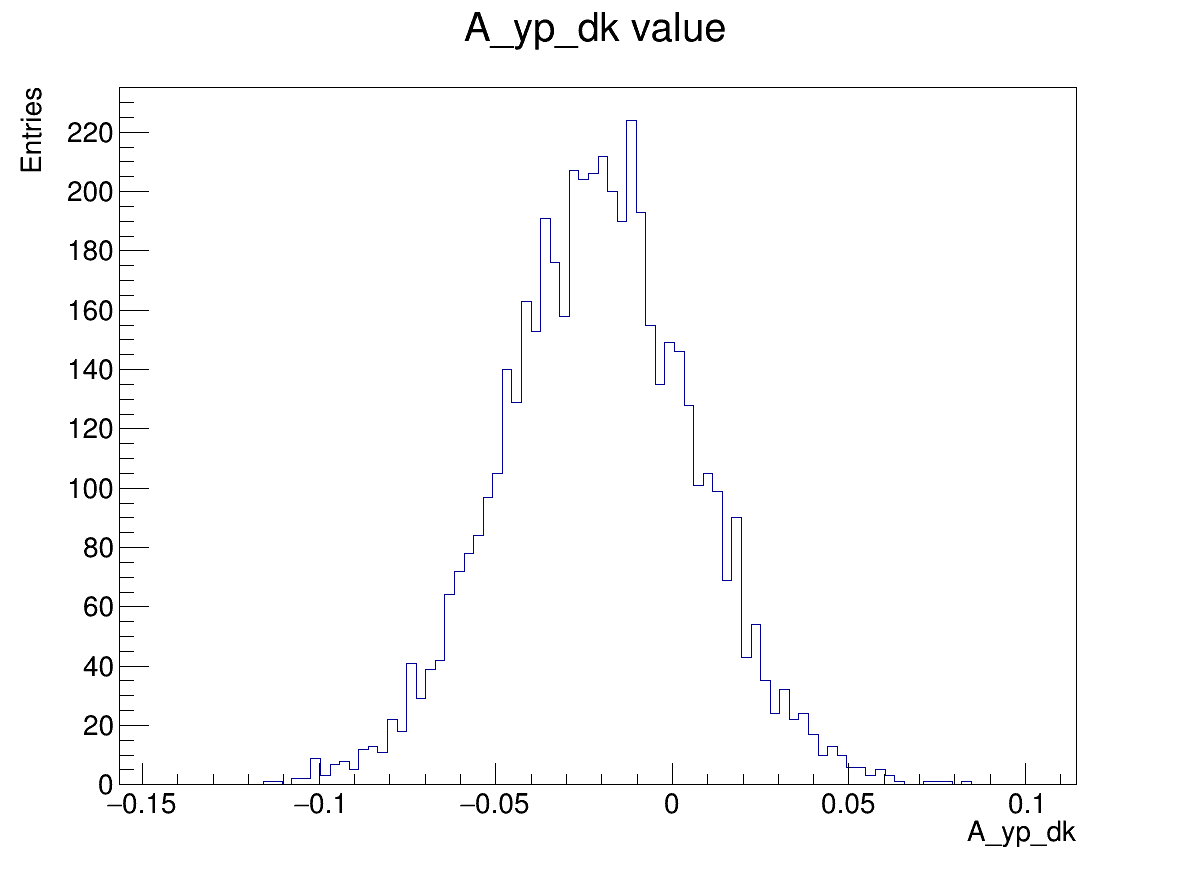
\includegraphics[width = 1.0\textwidth]{Plots/A_yp_dk_value.png}
    \end{subfigure}
    \begin{subfigure}{0.42\textwidth}
      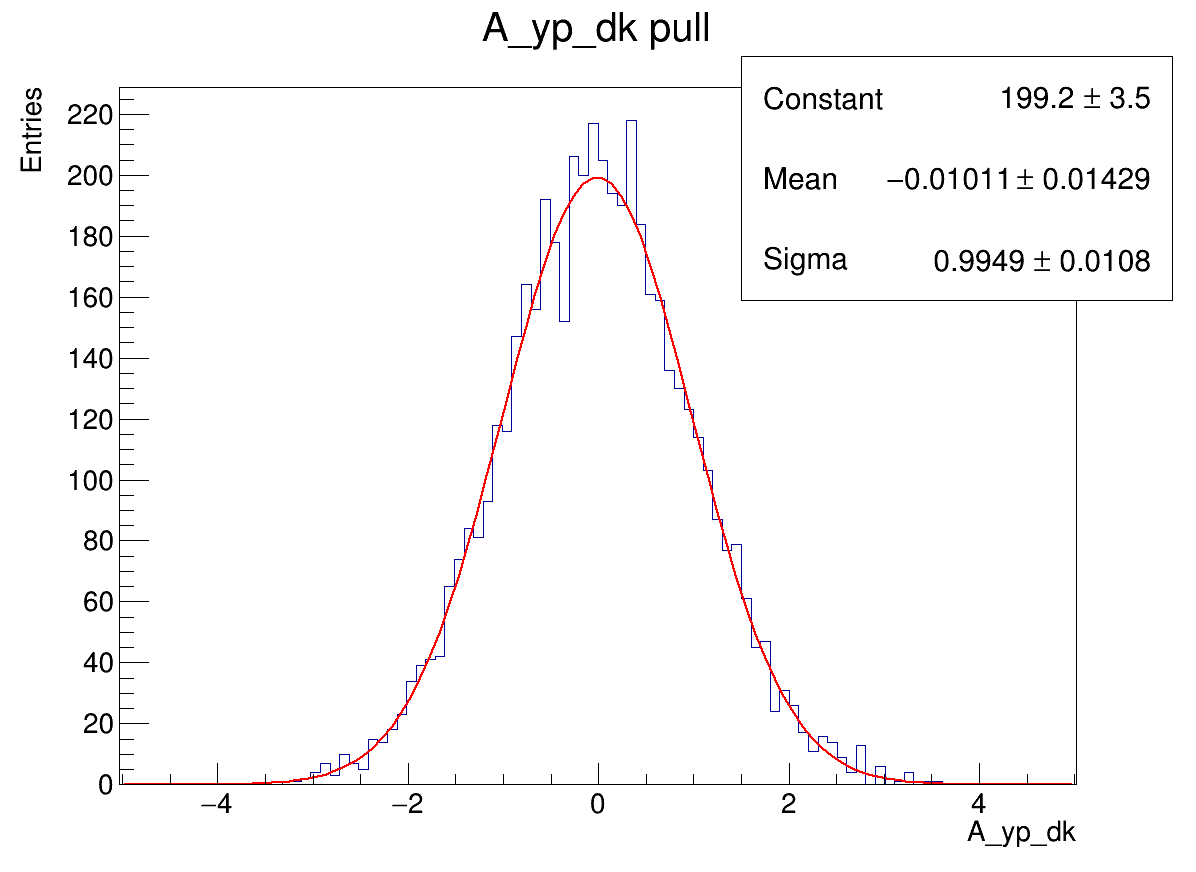
\includegraphics[width = 1.0\textwidth]{Plots/A_yp_dk_pull.png}
    \end{subfigure}%
    \begin{subfigure}{0.42\textwidth}
      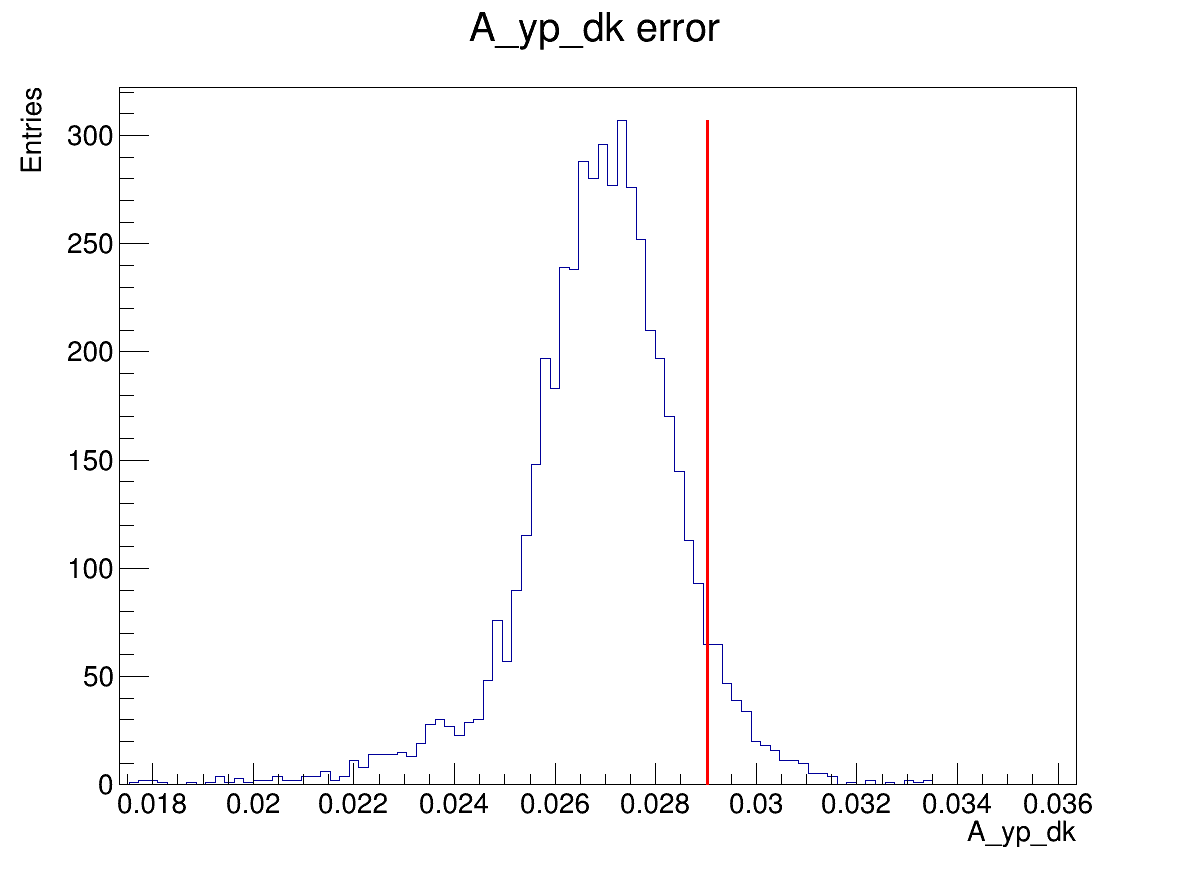
\includegraphics[width = 1.0\textwidth]{Plots/A_yp_dk_error_WithDataUncertainty.png}
    \end{subfigure}
  \end{figure}
\end{frame}

\begin{frame}{CP observables result: $x_\xi^{D\pi}$}
  \begin{figure}
    \centering
    \begin{subfigure}{0.42\textwidth}
      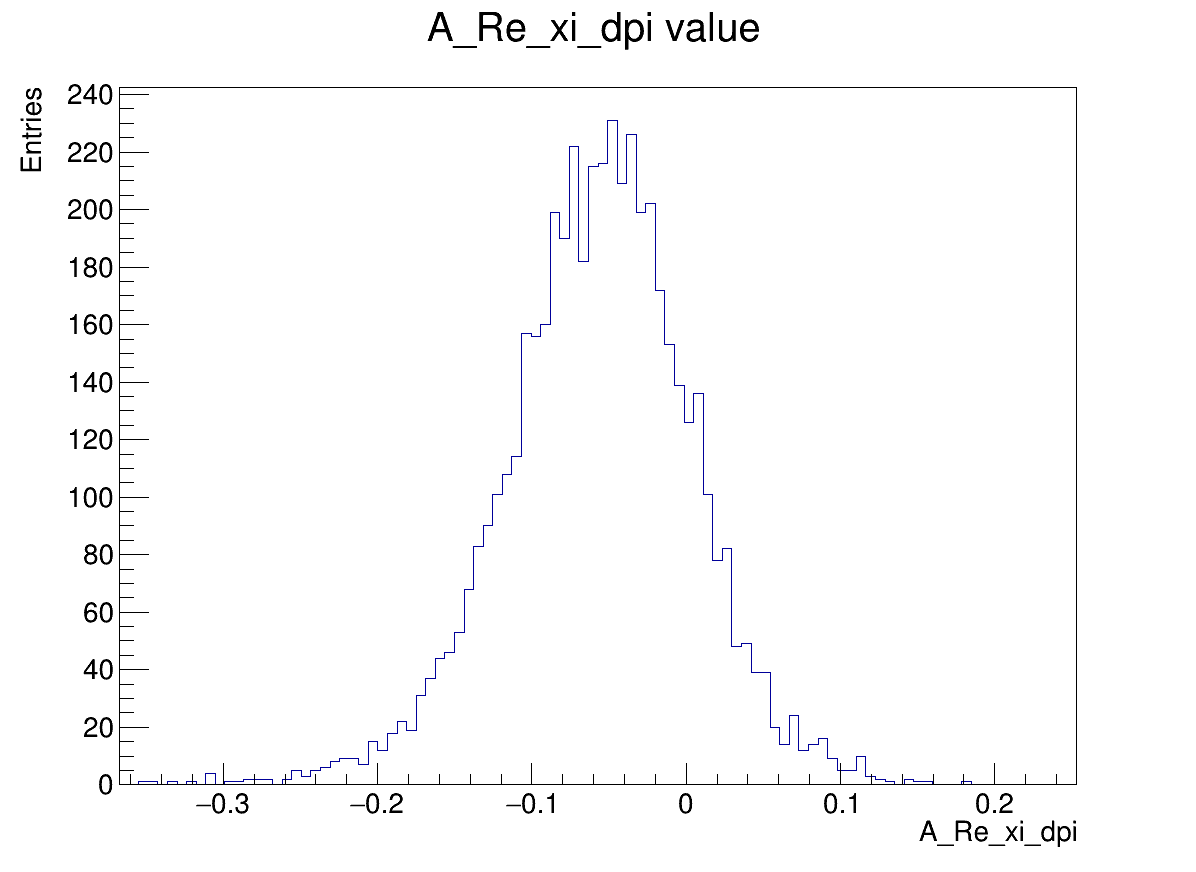
\includegraphics[width = 1.0\textwidth]{Plots/A_Re_xi_dpi_value.png}
    \end{subfigure}
    \begin{subfigure}{0.42\textwidth}
      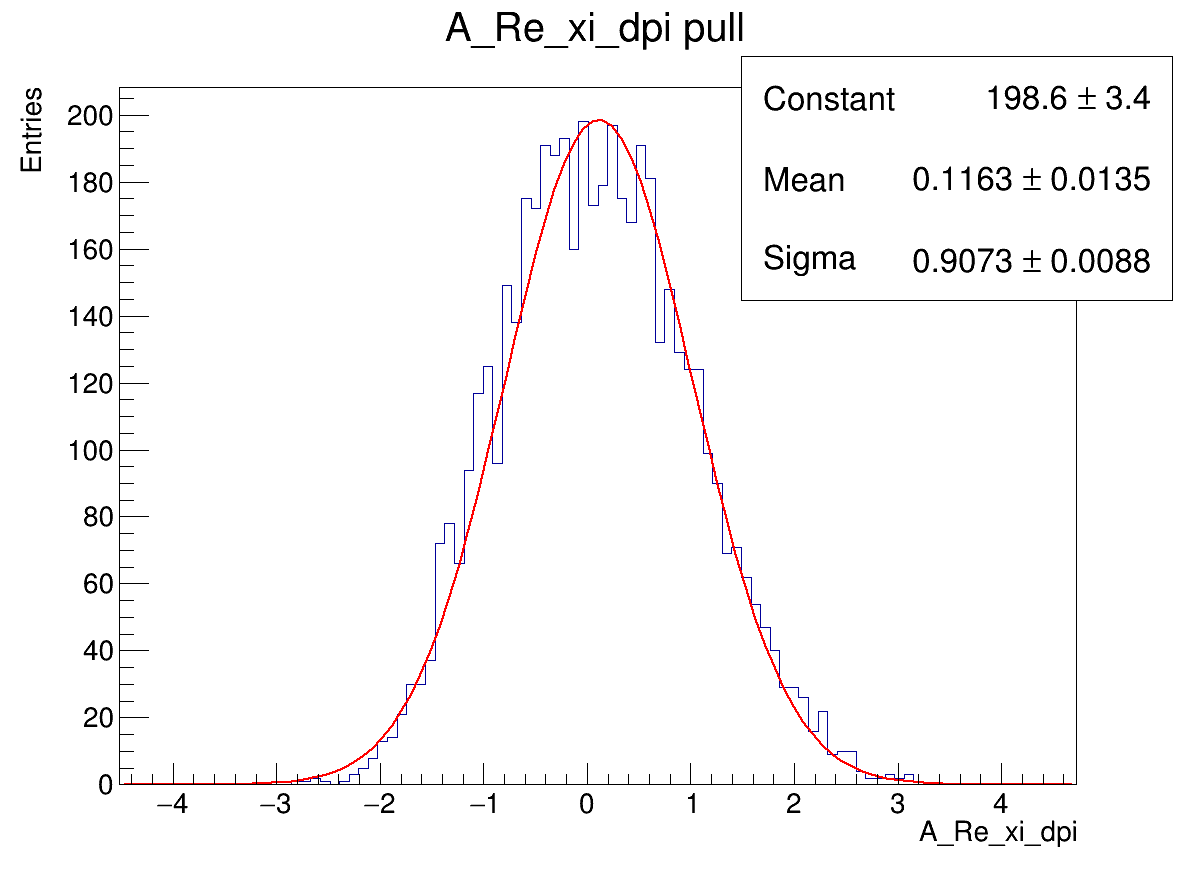
\includegraphics[width = 1.0\textwidth]{Plots/A_Re_xi_dpi_pull.png}
    \end{subfigure}%
    \begin{subfigure}{0.42\textwidth}
      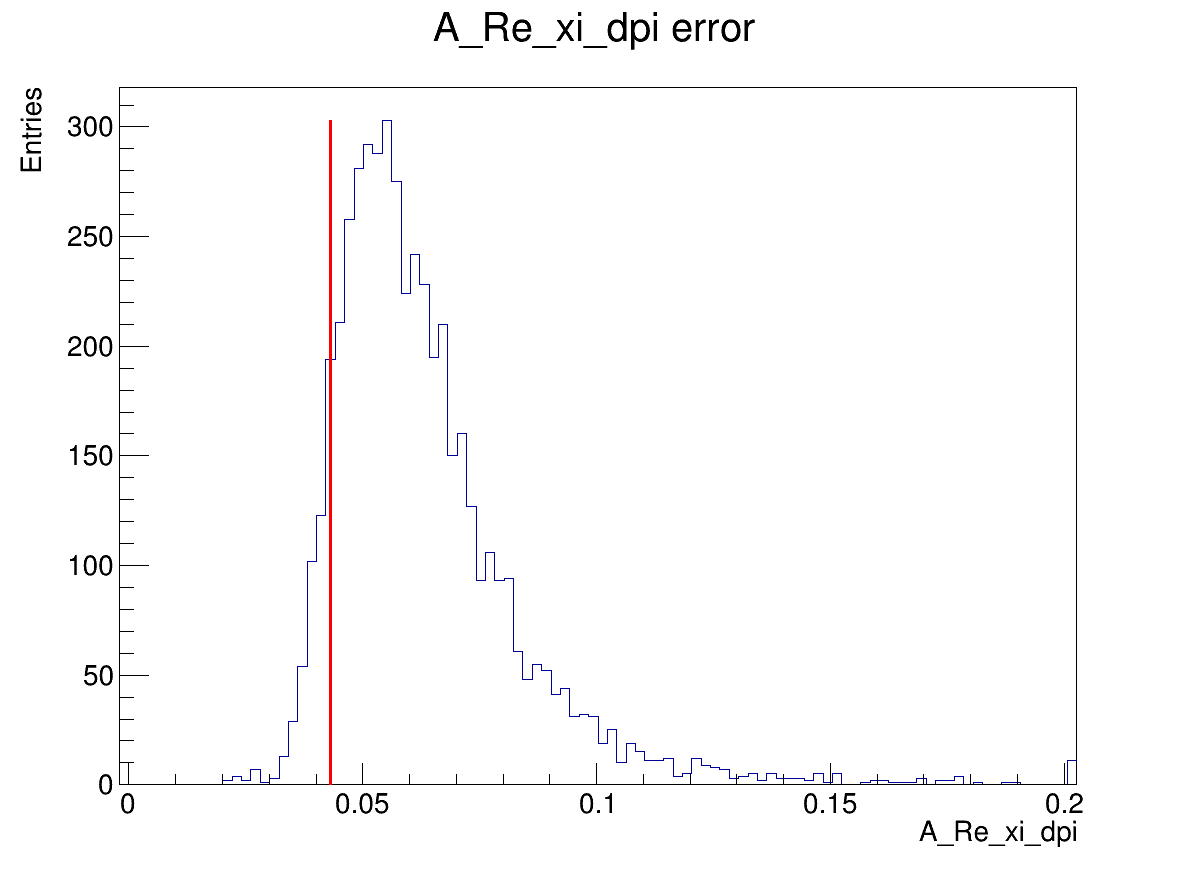
\includegraphics[width = 1.0\textwidth]{Plots/A_Re_xi_dpi_error_WithDataUncertainty.png}
    \end{subfigure}
  \end{figure}
\end{frame}

\begin{frame}{CP observables result: $y_\xi^{D\pi}$}
  \begin{figure}
    \centering
    \begin{subfigure}{0.42\textwidth}
      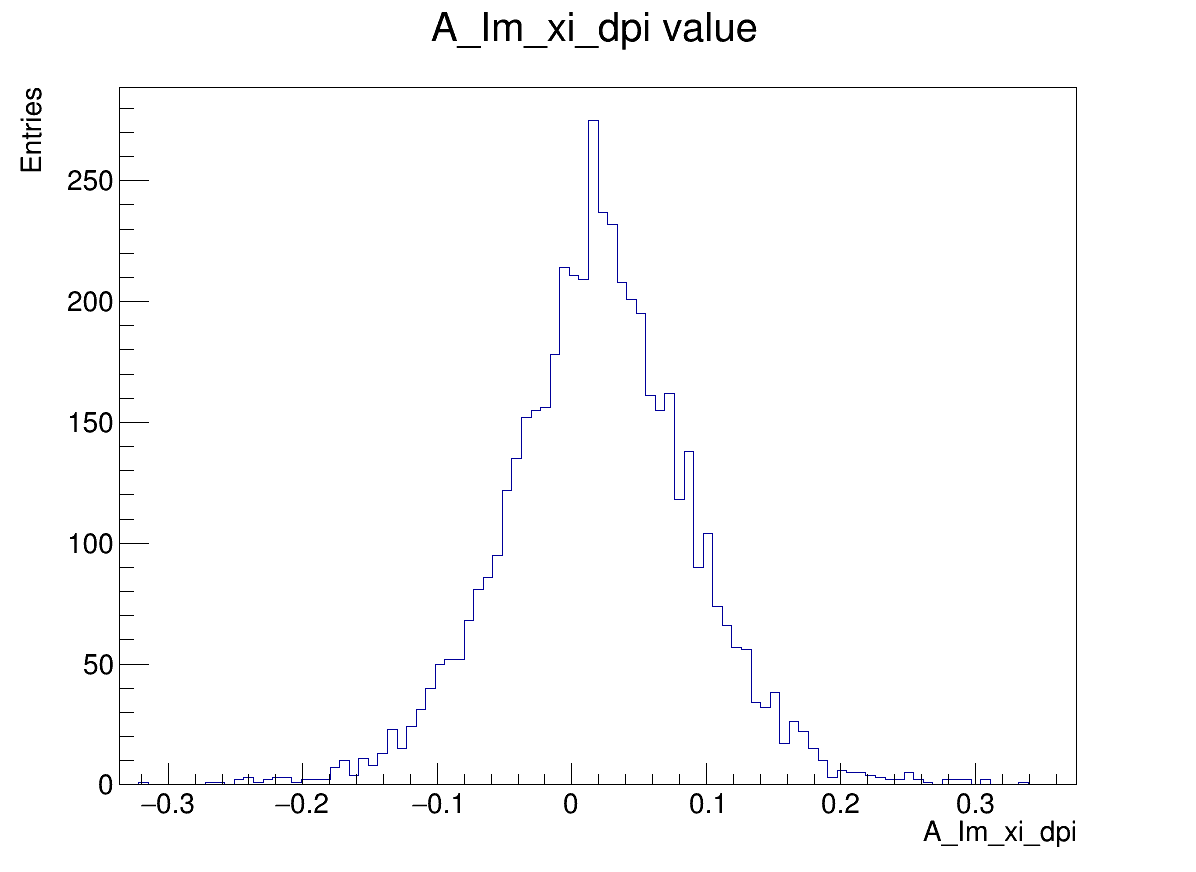
\includegraphics[width = 1.0\textwidth]{Plots/A_Im_xi_dpi_value.png}
    \end{subfigure}
    \begin{subfigure}{0.42\textwidth}
      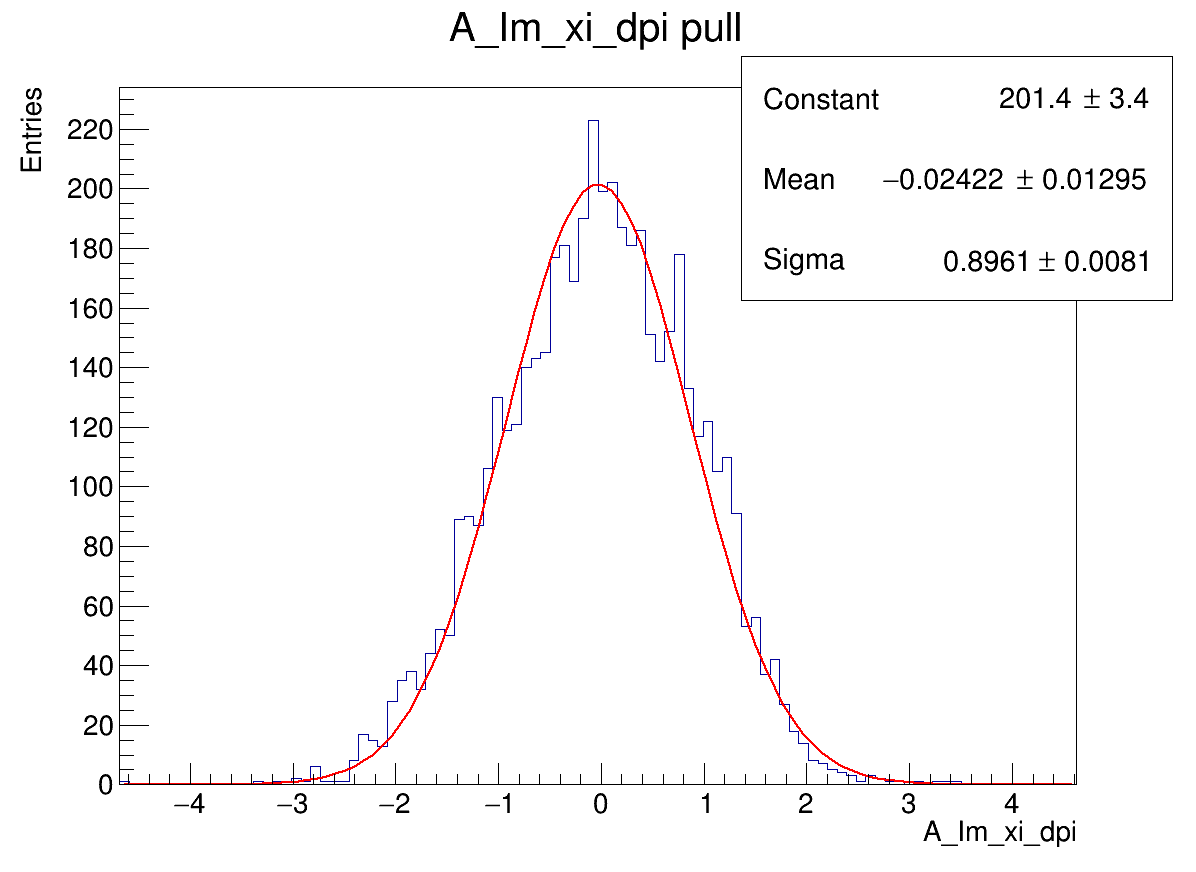
\includegraphics[width = 1.0\textwidth]{Plots/A_Im_xi_dpi_pull.png}
    \end{subfigure}%
    \begin{subfigure}{0.42\textwidth}
      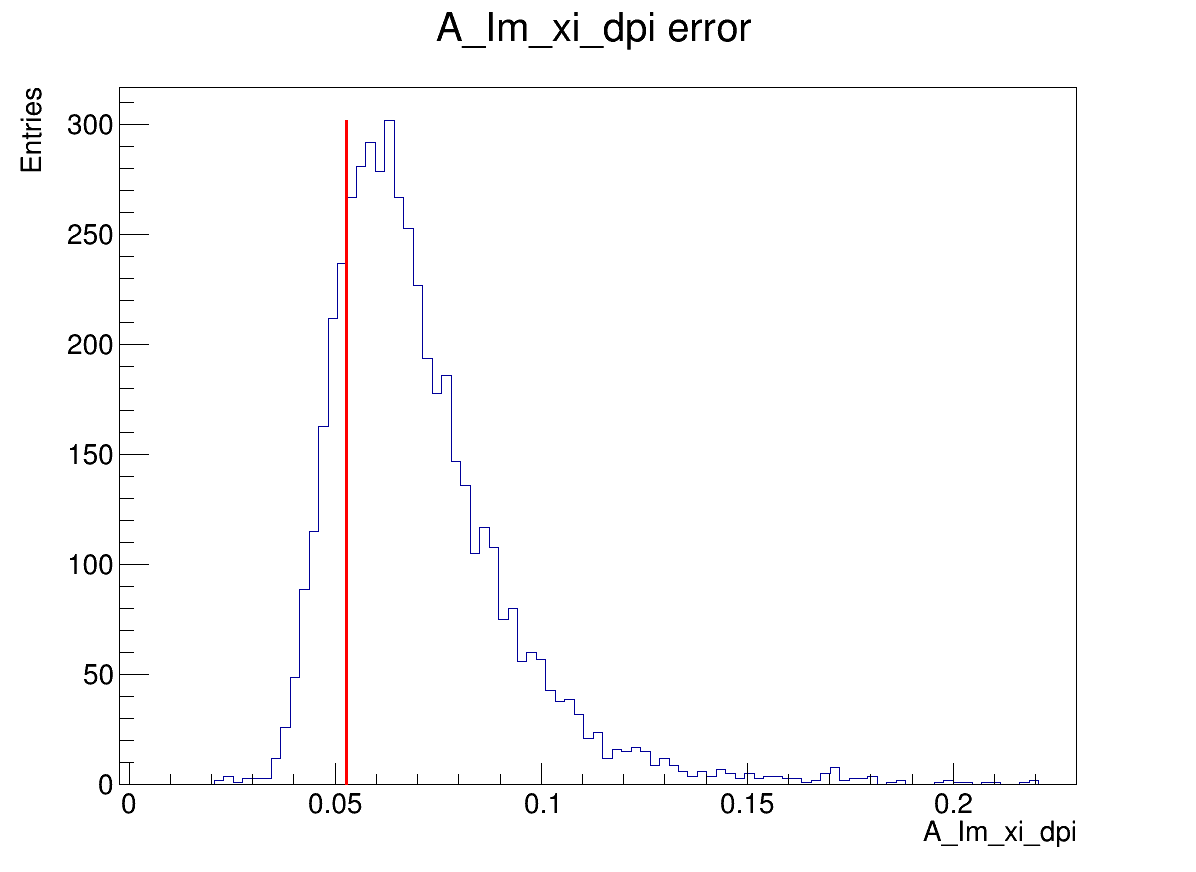
\includegraphics[width = 1.0\textwidth]{Plots/A_Im_xi_dpi_error_WithDataUncertainty.png}
    \end{subfigure}
  \end{figure}
\end{frame}

\section{Systematic uncertainty}
\begin{frame}{Systematic uncertainties}
  \begin{center}
    {\huge Systematic uncertainties}
  \end{center}
\end{frame}

\begin{frame}{$c_i$ and $s_i$ systematic uncertainty}
  \begin{itemize}
    \setlength\itemsep{1.5em}
    \item{Uncertainty of $c_i$ and $s_i$ in BESIII analysis (mostly statistical)}
    \item{Largest systematic uncertainty}
    \item{Take uncertainties from $D\to4\pi$ strong phase analysis and extrapolate to $\SI{20}{\per\femto\barn}$}
    \item{Smear $c_i$ and $s_i$ and do many fits to data}
  \end{itemize}
\end{frame}

\begin{frame}{Remaining systematic uncertainties}
  Different strategies for evaluating systematic uncertainties:
  \vspace{0.2cm}
  \begin{itemize}
    \setlength\itemsep{1em}
    \item{Generate toy datasets with systematics, fit with default model and take the bias as a systematic:}
    \begin{itemize}
      \item{Small backgrounds ($D\to K(X)l\nu_l$, $D\to K\pi\pi\pi$, $B\to Dl\nu_l$, $\Lambda_b$)}
      \item{Bin dependent mass shape}
      \item{Low mass physics effects}
    \end{itemize}
    \item{Do multiple fits to data while smearing parameters:}
    \begin{itemize}
      \item{$c_i$ and $s_i$}
      \item{Mass shape}
      \item{Fixed yield fractions}
      \item{PID efficiency}
    \end{itemize}
    \item{Fit bias: Take bias toys as systematic uncertainty}
  \end{itemize}
\end{frame}

\begin{frame}{Summary of all systematic uncertainties}
  \begin{tabular}{lcccccc} 
        \hline
        Source & $x_-^{DK}$ & $y_-^{DK}$ & $x_+^{DK}$ & $y_+^{DK}$ & $x_\xi^{D\pi}$ & $y_\xi^{D\pi}$ \\
        \hline
        Statistical                              & 2.73  & 3.23  & 2.38  & 2.90  & 4.30  & 5.27  \\
        \hline
        $c_i$, $s_i$                             & 0.66  & 1.55  & 0.32  & 1.31  & 1.73  & 1.03  \\
        \hline
        $B^\pm\to D\mu\nu$ background            & 0.04  & 0.03  & 0.02  & 0.15  & 0.30  & 0.10 \\
        $D\to K(X)l\nu_l$ background             & 0.15  & 0.05  & 0.11  & 0.03  & 0.35  & 0.25 \\
        $D\to K\pi\pi\pi$ background             & 0.17  & 0.03  & 0.04  & 0.01  & 0.46  & 0.18 \\
        $\Lambda_b$ background                   & 0.09  & 0.11  & 0.00  & 0.18  & 0.16  & 0.21 \\
        Bin dependent mass shape                 & 0.21  & 0.05  & 0.17  & 0.01  & 0.37  & 0.11 \\
        Fit bias                                 & 0.19  & 0.03  & 0.16  & 0.04  & 0.30  & 0.16 \\
        Fixed yield fractions                    & 0.02  & 0.03  & 0.02  & 0.02  & 0.01  & 0.01 \\
        Low mass physics effects                 & 0.05  & 0.09  & 0.05  & 0.18  & 0.41  & 0.48 \\
        Mass shape                               & 0.03  & 0.03  & 0.02  & 0.02  & 0.04  & 0.01 \\
        PID Efficiency                           & 0.03  & 0.03  & 0.02  & 0.02  & 0.04  & 0.01 \\
        \hline
        Total LHCb systematic                    & 0.39  & 0.17  & 0.27  & 0.30  & 0.92  & 0.65  \\
        \hline
        Total systematic                         & 0.77  & 1.55  & 0.41  & 1.34  & 1.96  & 1.22  \\
        \hline
  \end{tabular}
\end{frame}

\section{Summary and conclusion}
\begin{frame}{Summary and conclusion}
  \begin{center}
    {\huge Summary and conclusion}
  \end{center}
\end{frame}

\begin{frame}{Summary of CP observables}
  \begin{itemize}
    \item{Measured CP observables:}
  \end{itemize}
  \begin{align*}
    x_-^{DK} =& (x.x \pm 2.7 \pm 0.4 \pm 0.7)\times 10^{-2}, \\
    y_-^{DK} =& (x.x \pm 3.2 \pm 0.2 \pm 1.6)\times 10^{-2}, \\
    x_+^{DK} =& (x.x \pm 2.4 \pm 0.3 \pm 0.3)\times 10^{-2}, \\
    y_+^{DK} =& (x.x \pm 2.9 \pm 0.3 \pm 1.3)\times 10^{-2}, \\
    x_\xi^{D\pi} =& (x.x \pm 4.3 \pm 0.9 \pm 1.7)\times 10^{-2}, \\
    y_\xi^{D\pi} =& (x.x \pm 5.3 \pm 0.6 \pm 1.0)\times 10^{-2},
  \end{align*}
  \vspace{-0.5cm}
  \begin{itemize}
    \item{Note: Currently using $c_i$ and $s_i$ from the \underline{LHCb model}}
    \item{Publication strategy: Publish current results together with binned yields $\to$ Redo fit to obtain model-independent CP observables once $c_i$ and $s_i$ from BESIII are available}
  \end{itemize}
\end{frame}

\begin{frame}{Interpretation in terms of $\gamma$}
  \begin{itemize}
    \item{Interpret in terms of physics parameters:}
  \end{itemize}
  \begin{align*}
    \gamma &= (x.x^{+14}_{-15})^\circ, \\
    \delta_B^{DK} &= (x.x^{+15}_{-14})^\circ, \\
    r_B^{DK} &= x.x^{+0.019}_{-0.018}, \\
    \delta_B^{D\pi} &= (x.x^{+117}_{-63})^\circ, \\
    r_B^{D\pi} &= x.x^{+0.0052}_{-0.0024}.
  \end{align*}
\end{frame}

\begin{frame}{Bonus measurement}
  \begin{itemize}
    \setlength\itemsep{1em}
    \item{The mode $B^\pm\to Dh^\pm$, $D\to\pi^+\pi^-\pi^+\pi^-$ very similar}
    \item{Run this through \underline{same} selection (including BDT)}
    \item{Can measure GLW CP observables as additional constraints on $\gamma$:}
  \end{itemize}
  \begin{align*}
    A_h =& \frac{\Gamma(B^-\to Dh^-) - \Gamma(B^+\to Dh^+)}{\Gamma(B^-\to Dh^-) + \Gamma(B^+\to Dh^+)}, \\
    R_{\rm CP} =& \frac{R(4\pi)}{R(K3\pi)}, \\
    R =& \frac{\Gamma(B\to DK)}{\Gamma(B\to D\pi)}.
  \end{align*}
  \begin{itemize}
    \item{$B^\pm\to Dh^\pm$, $D\to K\pi\pi\pi$ yields provided by Tim Evans}
  \end{itemize}
\end{frame}

\begin{frame}{Global fit of $B^\pm\to Dh^\pm$, $D\to\pi^+\pi^-\pi^+\pi^-$}
  \vspace{-0.3cm}
  \begin{figure}
    \centering
    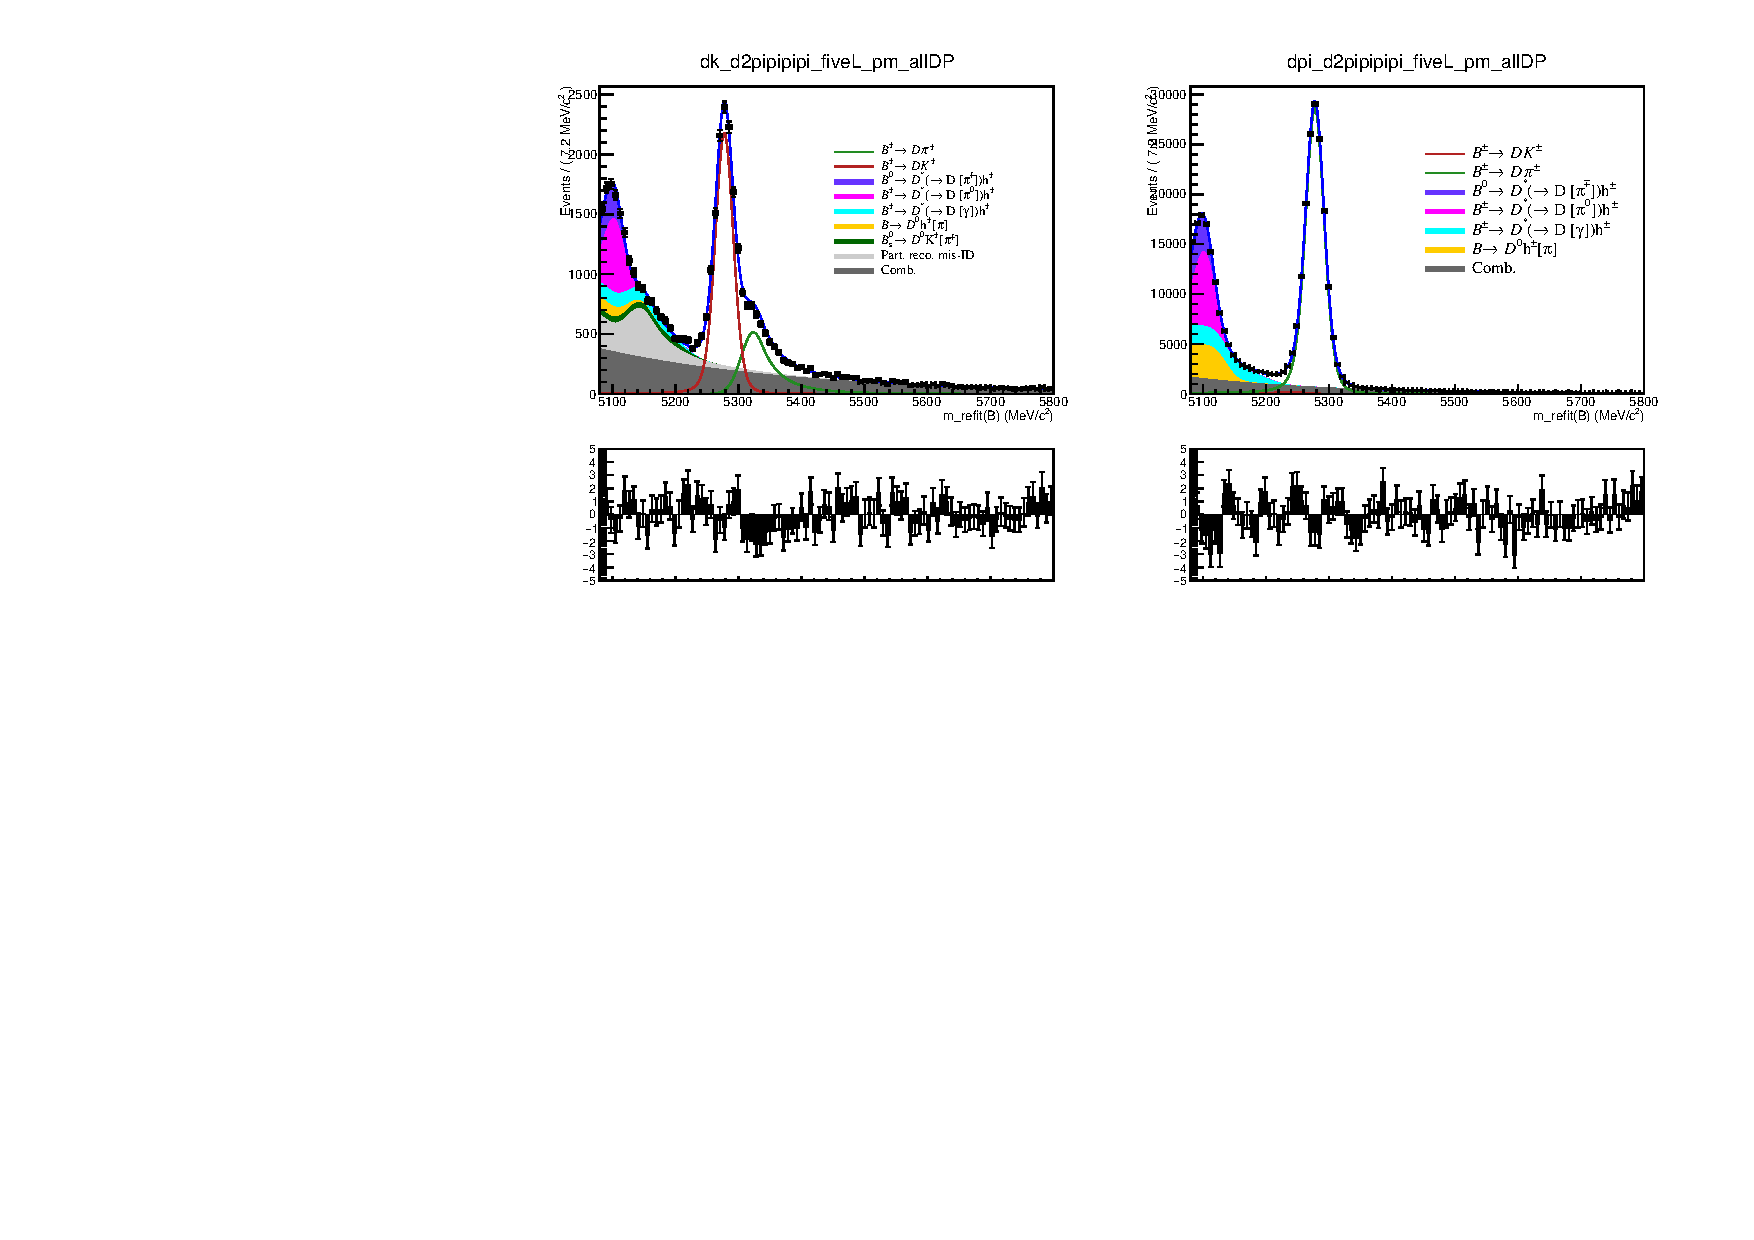
\includegraphics[width = 1.0\textwidth]{Plots/d2pipipipi_fiveL_allDP.pdf}
  \end{figure}
  \vspace{-0.2cm}
  \begin{equation*}
    \frac{{\rm Yield}(\pi\pi\pi\pi)}{{\rm Yield}(KK\pi\pi)} = \frac{\SI{161900(455)}{}}{\SI{54039(256)}{}} = \SI{2.996(17)}{}
  \end{equation*}
  \begin{center}
    Compare with PDG: $\SI{3.06(16)}{}$
  \end{center}
\end{frame}

\begin{frame}{Thank you!}
  \begin{center}
    {\huge Thank you!}
  \end{center}
\end{frame}

\begin{frame}{Backup}
  \begin{center}
    {\huge Backup}
  \end{center}
\end{frame}

\begin{frame}{Binning scheme}
  \begin{figure}
    \centering
    \vspace{-0.2cm}
    \begin{subfigure}{0.5\textwidth}
      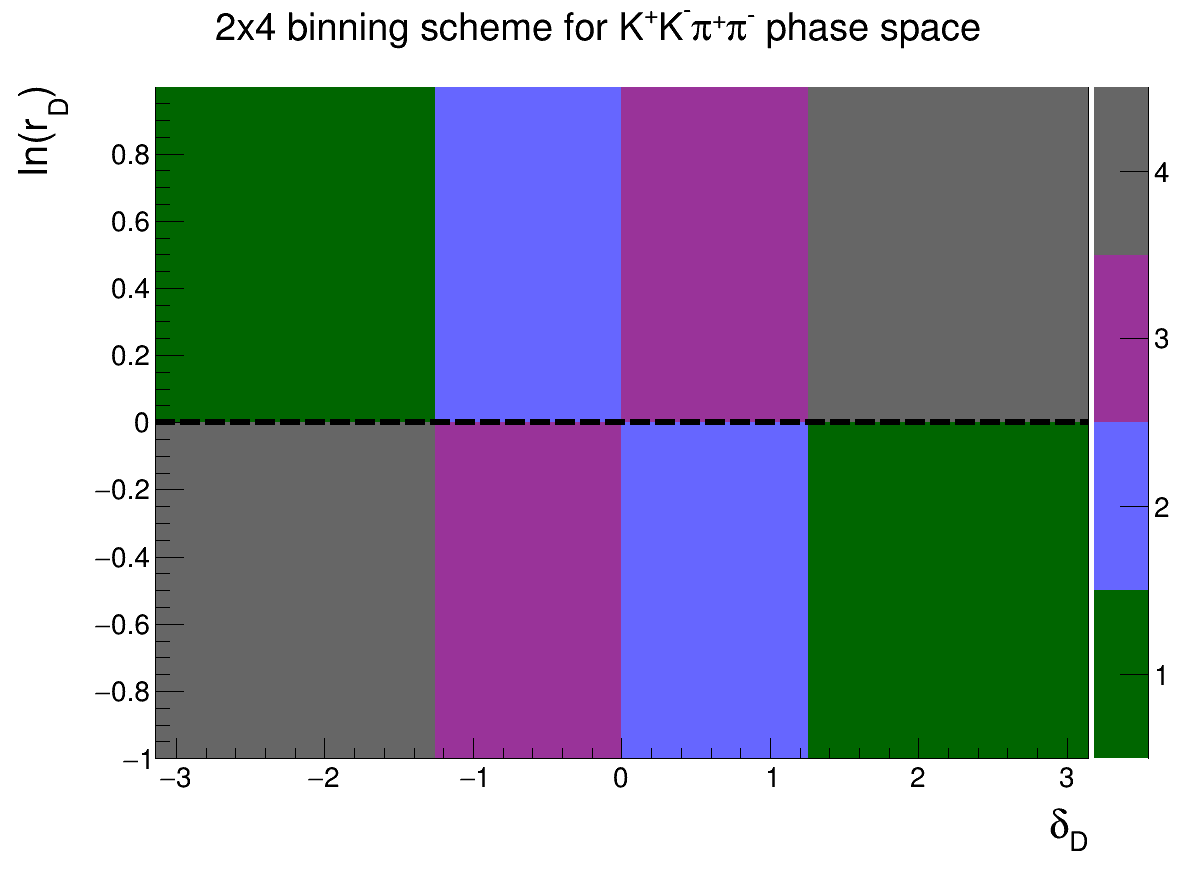
\includegraphics[width = 1.0\textwidth]{Plots/BinningSchemePlot_4Bins.png}
      \caption{$Q = 0.85$}
    \end{subfigure}%
    \begin{subfigure}{0.5\textwidth}
      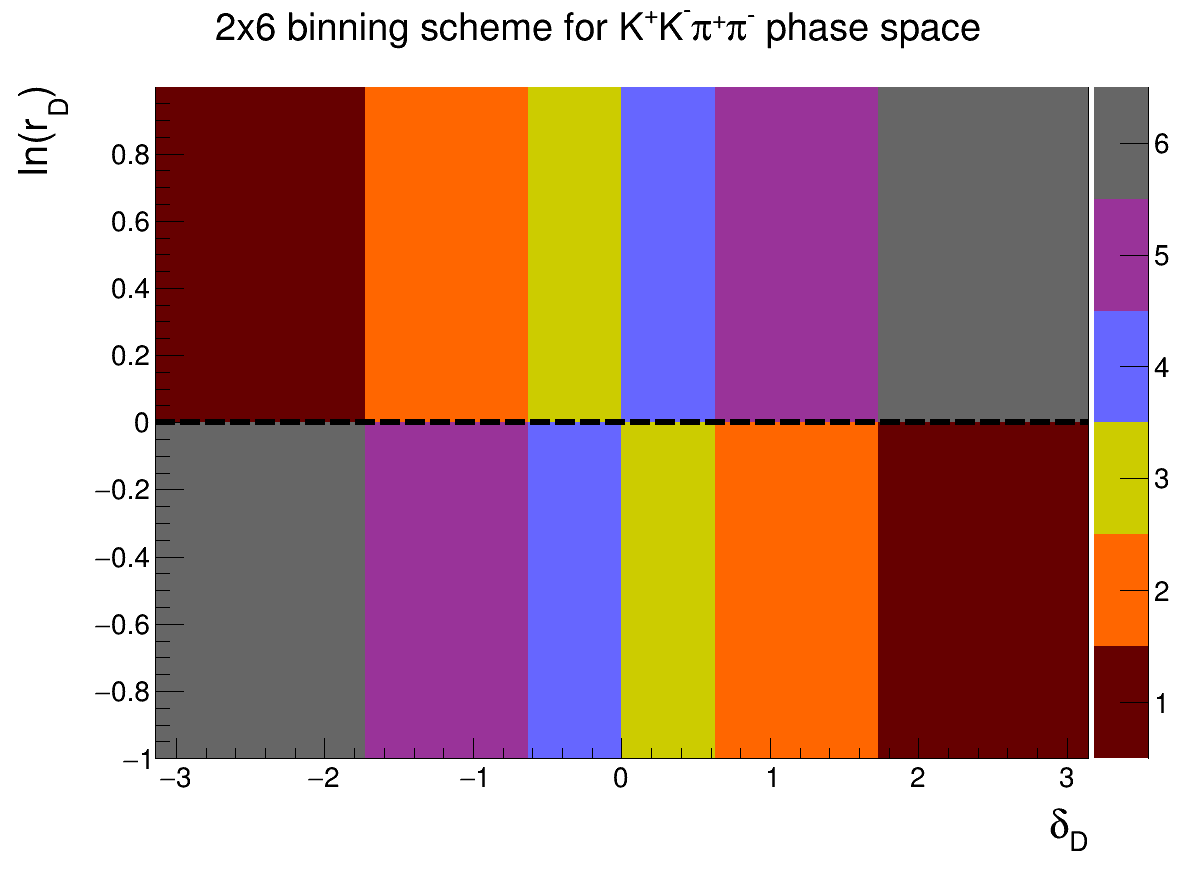
\includegraphics[width = 1.0\textwidth]{Plots/BinningSchemePlot_6Bins.png}
      \caption{$Q = 0.89$}
    \end{subfigure}
  \end{figure}
\end{frame}

\begin{frame}{$c_i$, $s_i$ and $F_i$}
  \begin{figure}
    \centering
    \vspace{-0.2cm}
    \begin{subfigure}{0.425\textwidth}
      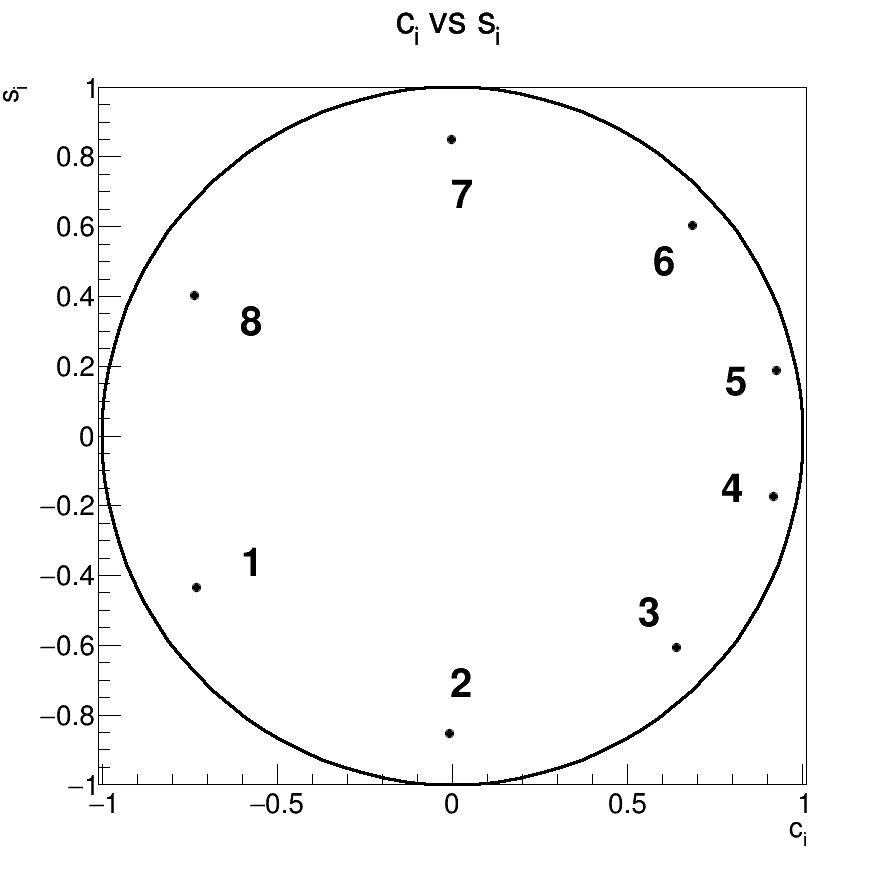
\includegraphics[width = 1.0\textwidth]{Plots/StrongPhaseParametersPlot_cisi_8Bins.png}
    \end{subfigure}%
    \begin{subfigure}{0.575\textwidth}
      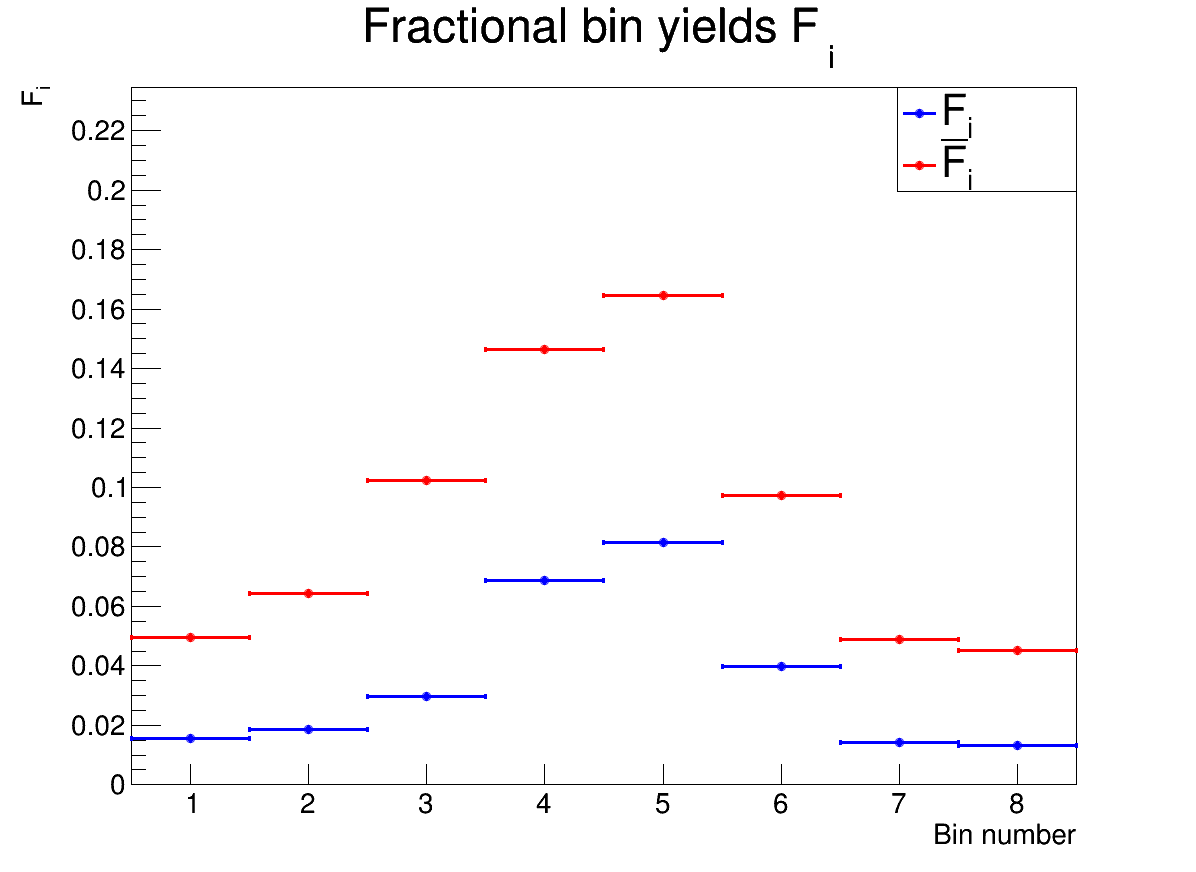
\includegraphics[width = 1.0\textwidth]{Plots/StrongPhaseParametersPlot_Fi_8Bins.png}
    \end{subfigure}
  \end{figure}
\end{frame}

\begin{frame}{Comparison of binned fit precision with unbinned fit}
  \begin{figure}
    \centering
    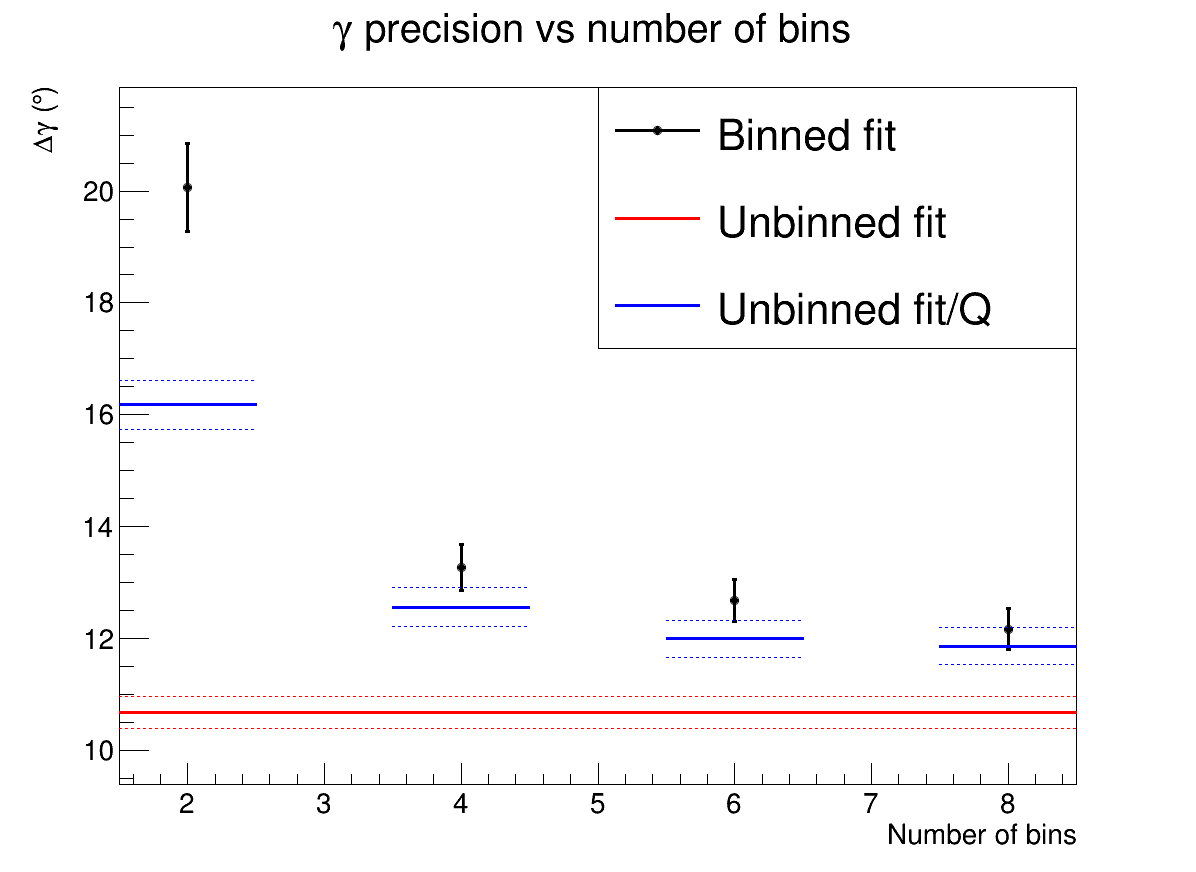
\includegraphics[width = 0.8\textwidth]{Plots/GammaPrecisionVersusBinNumber.png}
  \end{figure}
\end{frame}

\begin{frame}{Trigger requirements}
  \centering
  \def\arraystretch{1.2}%
  \begin{tabular}{|l|l|}
    \hline
    Run 1 trigger        & (\texttt{Bu\_L0Global\_TIS} or \texttt{Bu\_L0HadronDecision\_TOS}) \\
    requirements         & and (\texttt{Bu\_Hlt1TrackAllL0Decision\_TOS}) \\
                         & and (\texttt{Bu\_Hlt2Topo2BodyBBDTDecision\_TOS} or \\
                         & \texttt{Bu\_Hlt2Topo3BodyBBDTDecision\_TOS} or \\
                         & \texttt{Bu\_Hlt2Topo4BodyBBDTDecision\_TOS} or \\
                         & \texttt{Bu\_Hlt2IncPhiDecision\_TOS}) \\
    \hline
    Run 2 trigger        & (\texttt{Bu\_L0Global\_TIS} or \texttt{Bu\_L0HadronDecision\_TOS}) \\
    requirements         & and (\texttt{Bu\_Hlt1TrackMVADecision\_TOS} or \\
                         & \texttt{Bu\_Hlt1TwoTrackMVADecision\_TOS}) \\
                         & and (\texttt{Bu\_Hlt2Topo2BodyDecision\_TOS} or \\
                         & \texttt{Bu\_Hlt2Topo3BodyDecision\_TOS} or \\
                         & \texttt{Bu\_Hlt2Topo4BodyDecision\_TOS} or \\
                         & \texttt{Bu\_Hlt2IncPhiDecision\_TOS}) \\
    \hline
  \end{tabular}
\end{frame}

\begin{frame}{Initial cuts}
  \begin{center}
    Rectangular cuts before BDT
  \end{center}
  \centering
  \def\arraystretch{1.2}%
  \begin{tabular}{lllc} 
    \hline
    Number & Variable description   & Cut \\
    \hline
    $1$    & DTF converged          & True \\
    $2$    & Bachelor momentum      & $< 100\si{\giga\eV}$ \\
    $3$    & Bachelor has RICH      & True \\
    $4$    & $D$ invariant mass     & $[1839.84, 1889.84]\si{\mega\eV}$ \\
    $5$    & $B^\pm$ invariant mass & $[5080, 5800]\si{\mega\eV}$ \\
    $6$    & $K^\pm$ daughter PID   & $> -10$ \\
    $7$    & $\pi^\pm$ daughter PID & $< 20$ \\
    \hline
  \end{tabular}
\end{frame}

\begin{frame}{Final cuts}
  \begin{center}
    Rectangular cuts after BDT
  \end{center}
  \centering
  \def\arraystretch{1.2}%
  \begin{tabular}{lllc} 
    \hline
    Number & Variable description     & Cut \\
    \hline
    $8$    & $K^\pm$ bachelor PID     & $> 4$ \\
    $9$    & $\pi^\pm$ bachelor PID   & $< 4$ \\
    $10$   & Bachelor is muon         & False \\
    $11$   & $z$ flight significance  & $> 2$ \\
    $12$   & $K^\pm$ PID              & $> 0$ \\
    $13$   & $K_S^0$ mass veto        & $[477, 507]\si{\mega\eV}$ \\
    \hline
  \end{tabular}
\end{frame}

\begin{frame}{BDT training variables}
  \centering
  %\def\arraystretch{1.2}%
  \begin{tabular}{|l|l|l|}
    \hline
    Name & Rank ($\%$) & Description \\
    \hline
    \texttt{log(D0\_RHO\_BPV)} & $7.7$ & $D$ radial distance to beamline \\
    \texttt{log(Bu\_FDCHI2\_OWNPV)} & $6.3$ & $B^\pm$ flight distance $\chi^2$ \\
    \texttt{log(Bu\_RHO\_BPV)} & $6.1$ & $B^\pm$ radial distance to beamline \\
    \texttt{log(Bach\_PT)} & $6.1$ & Bachelor transverse momentum \\
    \texttt{Bu\_PTASY\_1.5} & $5.3$ & $B^\pm$ asymmetry parameter \\
    \texttt{log(1-D0\_DIRA\_BPV)} & $5.0$ & Angle between PV and $D$ \\
    \texttt{log(Bu\_IPCHI2\_OWNPV)} & $4.8$ & $B^\pm$ impact parameter $\chi^2$ \\
    \texttt{log(1-Bu\_DIRA\_BPV)} & $4.7$ & Angle between PV and $B^\pm$ \\
    \texttt{log(h[1,2]\_PT)} & $4.4$ & $K^\pm$ transverse momentum \\
    \texttt{Bu\_MAXDOCA} & $4.4$ & $B^\pm$ distance of closest approach \\
    \texttt{log(Bach\_IPCHI2\_OWNPV)} & $4.1$ & Bachelor impact parameter $\chi^2$ \\
    \hline
  \end{tabular}
\end{frame}

\begin{frame}{BDT training particles}
  \centering
  %\def\arraystretch{1.2}%
  \begin{tabular}{|l|l|l|}
    \hline
    Name & Rank ($\%$) & Description \\
    \hline
    \texttt{log(Bu\_constD0PV\_D0\_P)} & $3.7$ & $D$ momentum from DTF \\
    \texttt{log(D0\_VTXCHI2DOF)} & $3.3$ & $D0$ vertex fit $\chi^2$ \\
    \texttt{log(h[3,4]\_IPCHI2\_OWNPV)} & $3.3$ & $\pi^\pm$ impact parameter $\chi^2$ \\
    \texttt{log(D0\_IPCHI2\_OWNPV)} & $3.2$ & $D$ impact parameter $\chi^2$ \\
    \texttt{log(h[3,4]\_PT)} & $3.2$ & $\pi^\pm$ transverse momentum \\
    \texttt{log(Bu\_PT)} & $2.8$ & $B^\pm$ transverse momentum \\
    \texttt{log(h[1,2]\_P)} & $2.8$ & $K^\pm$ momentum \\
    \texttt{log(Bach\_P)} & $2.7$ & Bachelor momentum \\
    \texttt{log(Bu\_constD0PV\_P)} & $2.6$ & $B^\pm$ momentum from DTF \\
    \texttt{log(h[1,2]\_IPCHI2\_OWNPV)} & $2.5$ & $K^\pm$ impact parameter $\chi^2$ \\
    \texttt{D0\_MAXDOCA} & $2.5$ & $D$ distance of closest approach \\
    \texttt{log(Bu\_VTXCHI2DOF)} & $2.0$ & $B^\pm$ vertex fit $\chi^2$ \\
    \texttt{log(h[3,4]\_P)} & $1.9$ & $\pi^\pm$ momentum \\
    \hline
  \end{tabular}
\end{frame}

\begin{frame}{$D$ semileptonic backgrounds}
  \begin{itemize}
    \setlength\itemsep{1em}
    \item{$B^\pm\to Dh^\pm$, $D\to K(X)l\nu$, $K(X)\to K\pi\pi$}
    \begin{itemize}
      \item{$K_1(1270)$}
      \item{$K_1(1400)$}
      \item{$K^*(1410)$}
      \item{$K^*(1680)$}
      \item{$K_2^*(1430)$}
    \end{itemize}
    \item{Single mis-ID: $K\mu\pi\pi\to KK\pi\pi$}
    \item{Double mis-ID: $K\pi\pi\mu\to KK\pi\pi$}
    \item{Generate Rapidsim samples, reweight with PIDCalib2}
  \end{itemize}
\end{frame}

\begin{frame}{$D$ semileptonic backgrounds}
  \begin{figure}
    \centering
    \vspace{-0.2cm}
    \begin{subfigure}{0.5\textwidth}
      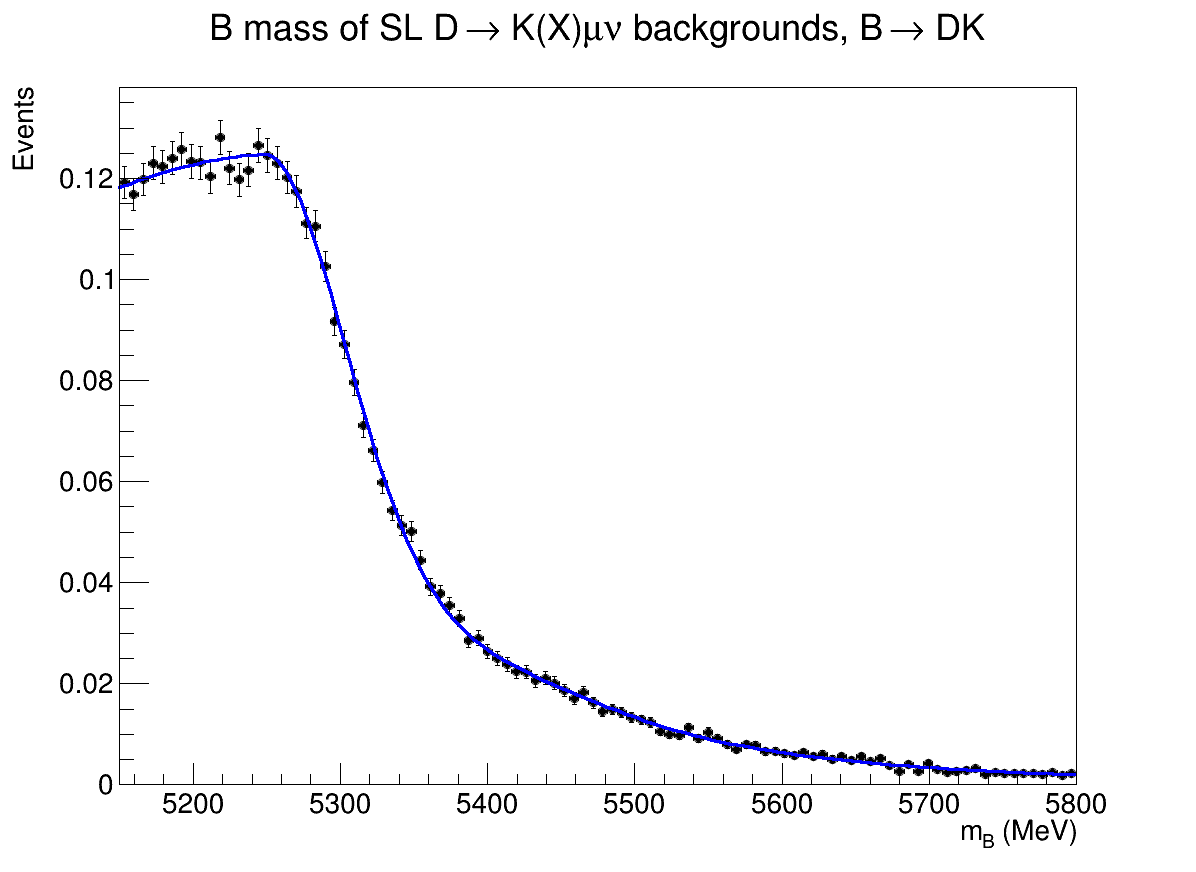
\includegraphics[width = 1.0\textwidth]{Plots/D_SL_RapidSim_Combined_Fit_B2DK.png}
      \caption{$B\to DK$}
    \end{subfigure}%
    \begin{subfigure}{0.5\textwidth}
      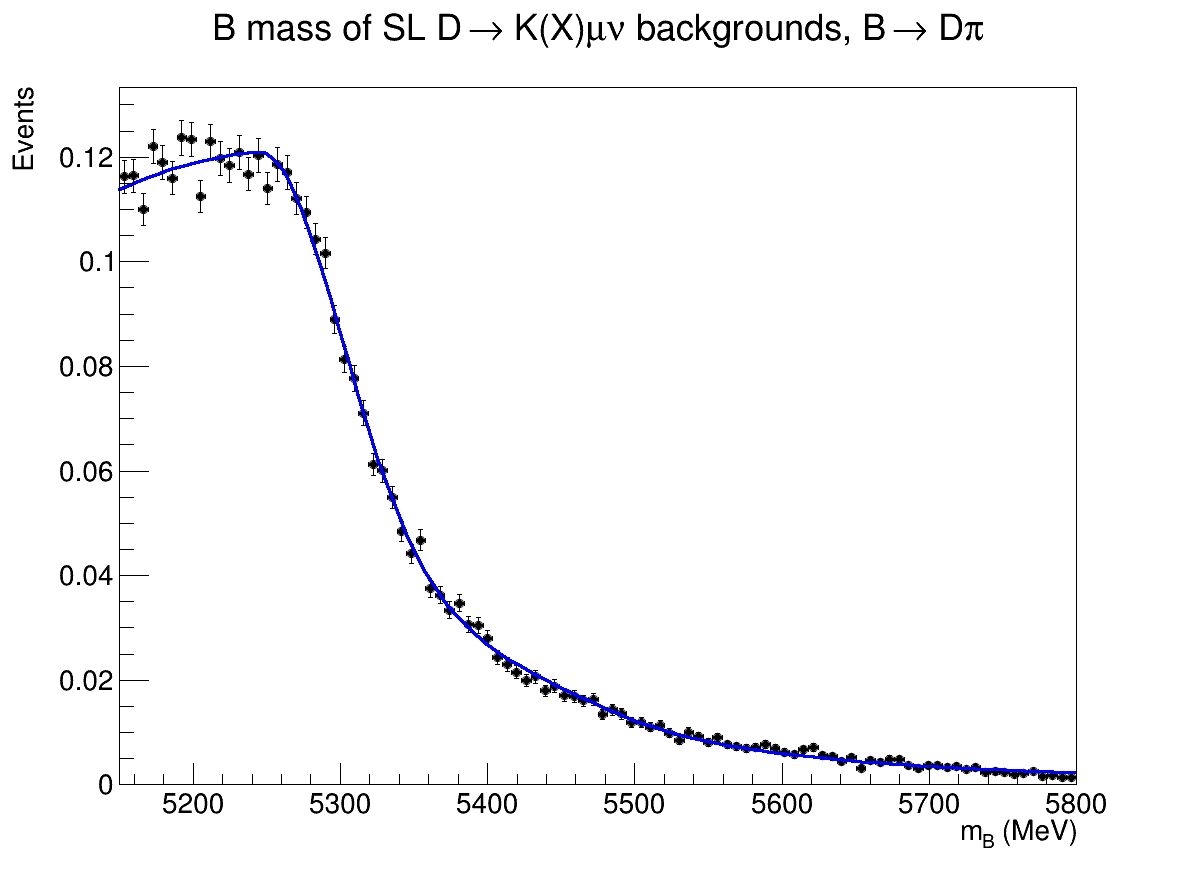
\includegraphics[width = 1.0\textwidth]{Plots/D_SL_RapidSim_Combined_Fit_B2Dpi.png}
      \caption{$B\to D\pi$}
    \end{subfigure}
  \end{figure}
  \begin{center}
    Conclusion: Negligible impact, include in systematics
  \end{center}
\end{frame}

\begin{frame}{Efficiency related systematics}
  Efficiency related systematics:
  \vspace{0.7cm}
  \begin{itemize}
    \setlength\itemsep{2em}
    \item{Difference in $B^\pm\to DK^\pm$ and $B^\pm\to D\pi^\pm$ phase space acceptance}
    \item{Efficiency correction of $c_i$ and $s_i$}
  \end{itemize}
\end{frame}

\begin{frame}{Efficiency differences between $B^\pm\to DK^\pm$ and $B^\pm\to D\pi^\pm$}
  \begin{figure}
    \centering
    \begin{subfigure}{0.33\textwidth}
      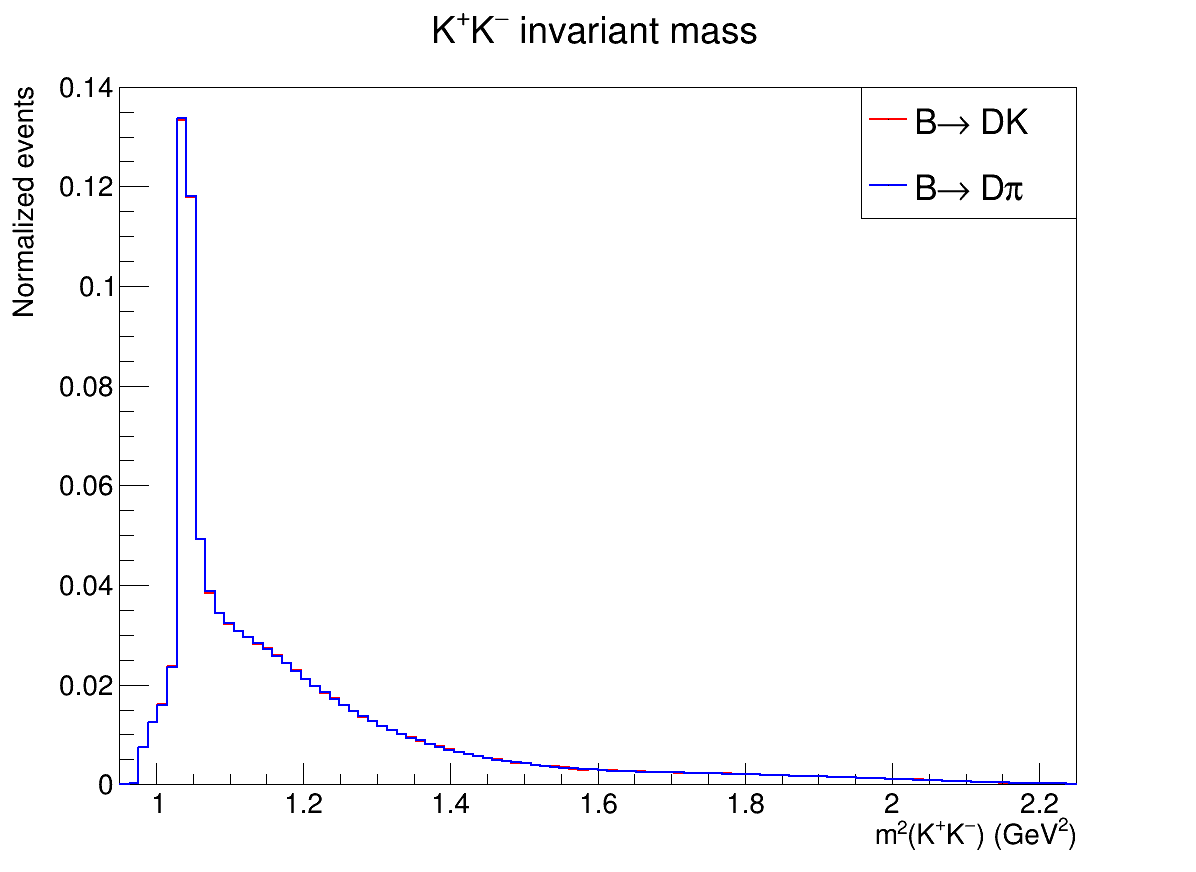
\includegraphics[width = 1.0\textwidth]{Plots/Dalitz_s01.png}
    \end{subfigure}%
    \begin{subfigure}{0.33\textwidth}
      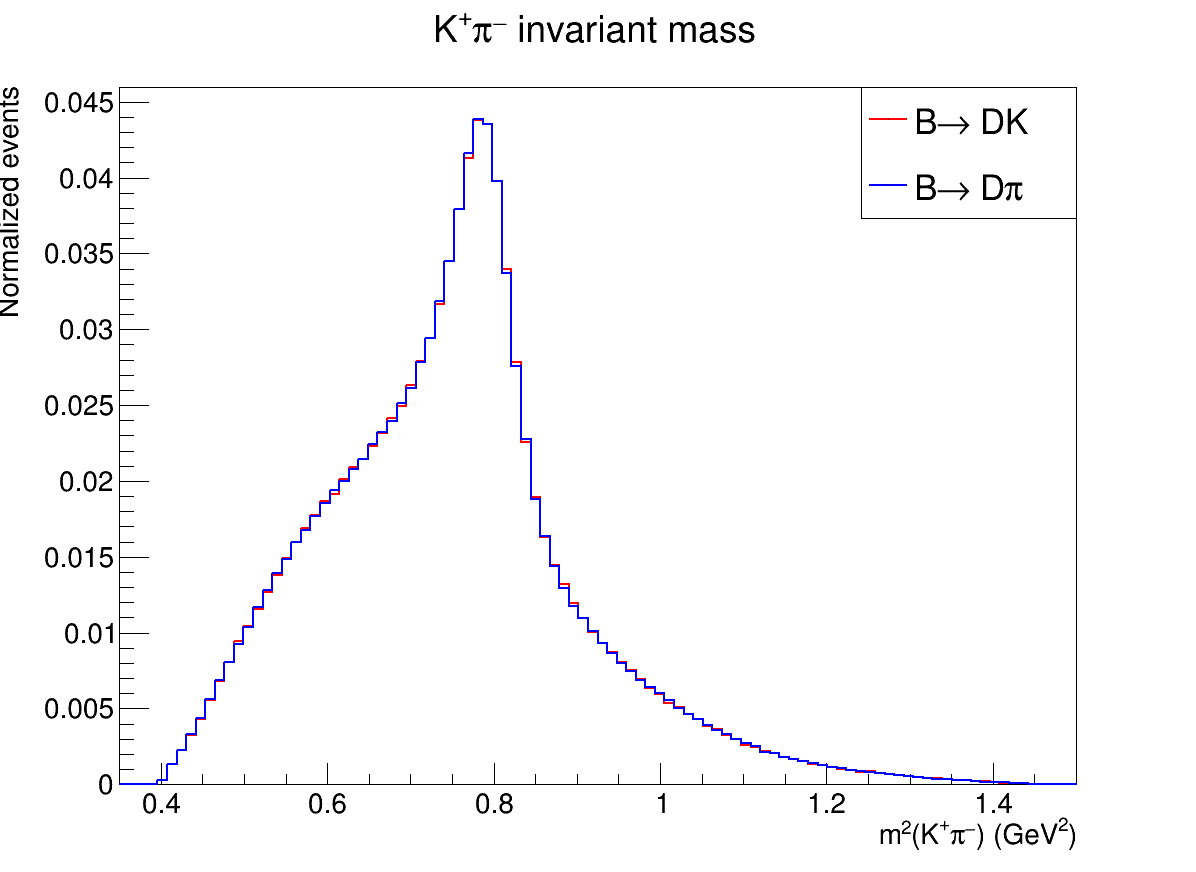
\includegraphics[width = 1.0\textwidth]{Plots/Dalitz_s03.png}
    \end{subfigure}%
    \begin{subfigure}{0.33\textwidth}
      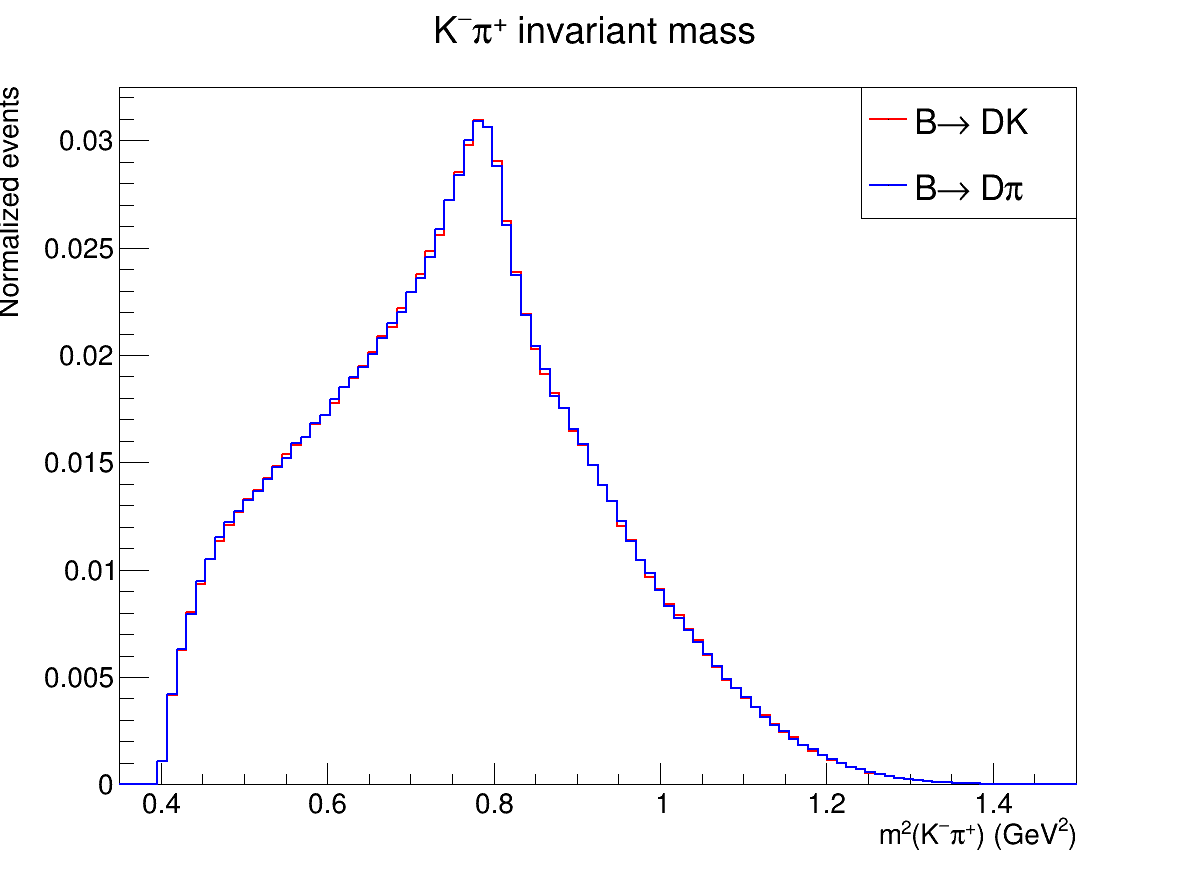
\includegraphics[width = 1.0\textwidth]{Plots/Dalitz_s12.png}
    \end{subfigure}
    \begin{subfigure}{0.33\textwidth}
      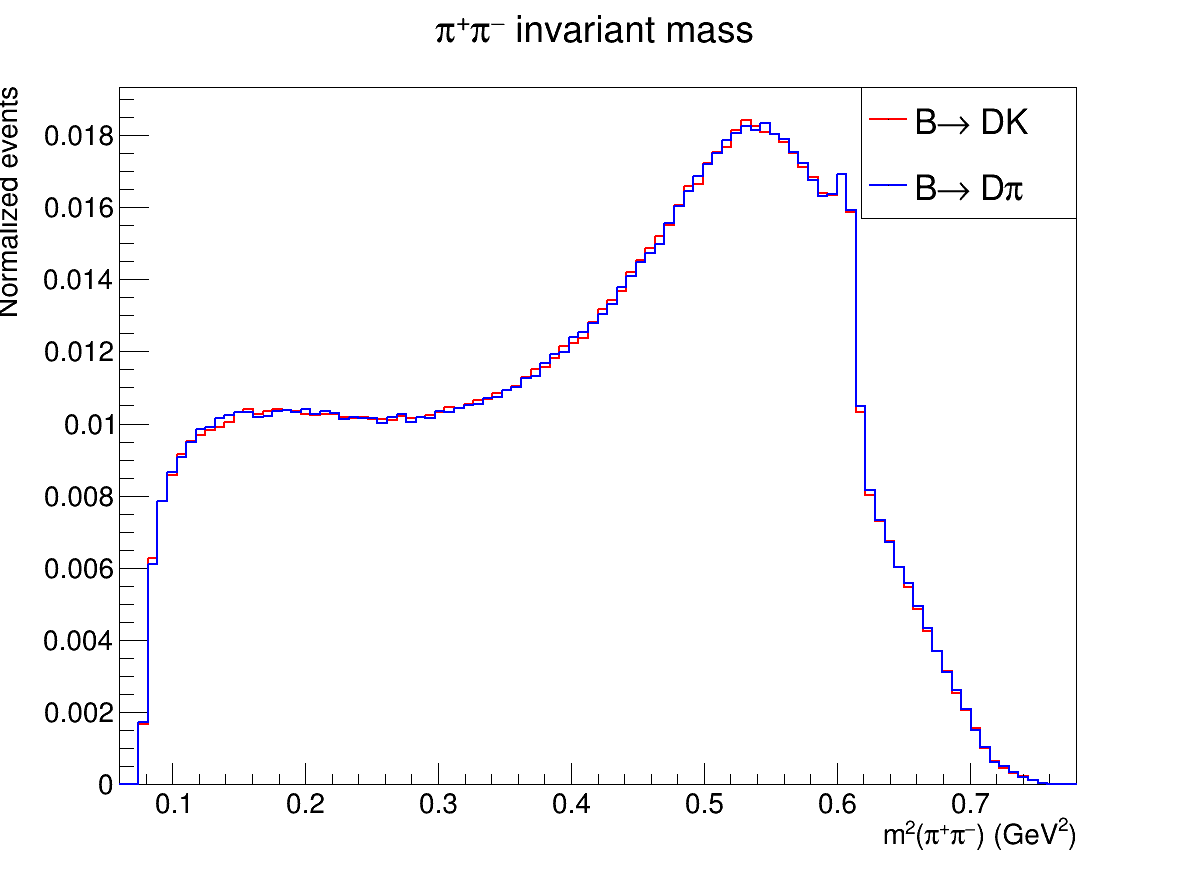
\includegraphics[width = 1.0\textwidth]{Plots/Dalitz_s23.png}
    \end{subfigure}%
    \begin{subfigure}{0.33\textwidth}
      \includegraphics[width = 1.0\textwidth]{Plots/Dalitz_s012.png}
    \end{subfigure}
  \end{figure}
  \begin{center}
    Conclusion: More or less identical phase space acceptance, no systematic uncertainty considered
  \end{center}
\end{frame}  

\begin{frame}{Efficiency correction of $c_i$ and $s_i$}
  \begin{figure}
    \centering
    \begin{subfigure}{0.33\textwidth}
      \includegraphics[width = 1.0\textwidth]{Plots/s01_BeforeReweighting.png}
    \end{subfigure}%
    \begin{subfigure}{0.33\textwidth}
      \includegraphics[width = 1.0\textwidth]{Plots/s03_BeforeReweighting.png}
    \end{subfigure}%
    \begin{subfigure}{0.33\textwidth}
      \includegraphics[width = 1.0\textwidth]{Plots/s12_BeforeReweighting.png}
    \end{subfigure}
    \begin{subfigure}{0.33\textwidth}
      \includegraphics[width = 1.0\textwidth]{Plots/s23_BeforeReweighting.png}
    \end{subfigure}%
    \begin{subfigure}{0.33\textwidth}
      \includegraphics[width = 1.0\textwidth]{Plots/s012_BeforeReweighting.png}
    \end{subfigure}
  \end{figure}
  \begin{center}
    Need to reweight events to account for efficiency differences between AmpGen samples and LHCb MC
  \end{center}
\end{frame}  

\begin{frame}{Efficiency correction of $c_i$ and $s_i$}
  \begin{figure}
    \centering
    \begin{subfigure}{0.33\textwidth}
      \includegraphics[width = 1.0\textwidth]{Plots/s01_AfterReweighting.png}
    \end{subfigure}%
    \begin{subfigure}{0.33\textwidth}
      \includegraphics[width = 1.0\textwidth]{Plots/s03_AfterReweighting.png}
    \end{subfigure}%
    \begin{subfigure}{0.33\textwidth}
      \includegraphics[width = 1.0\textwidth]{Plots/s12_AfterReweighting.png}
    \end{subfigure}
    \begin{subfigure}{0.33\textwidth}
      \includegraphics[width = 1.0\textwidth]{Plots/s23_AfterReweighting.png}
    \end{subfigure}%
    \begin{subfigure}{0.33\textwidth}
      \includegraphics[width = 1.0\textwidth]{Plots/s012_AfterReweighting.png}
    \end{subfigure}
  \end{figure}
  \begin{center}
    After reweighing, use weights to recalculate $c_i$ and $s_i$ \\
    Conclusion: Efficiency correction of $c_i$ and $s_i$ is an order of magnitude smaller than their uncertainties, no systematic uncertainty considered
  \end{center}
\end{frame}

\end{document}
